% master.tex : master-fil for projektet
% ------------------------------------------------------------------------------
% Dette er hovedfilen for projektet, hvori indhold fra alle input-filer (tekst,
% billeder, litteraturdatabaser, osv.) samles 

% Dokumenttypen 'book' er valgt pga. dens mange fleksible indstillinger
% Se https://tex.stackexchange.com/a/36989/118167
\documentclass[11pt,a4paper,oneside,openany,danish]{book}

% Variabler, som bruges til automatisk at indsætte titel, forfattere, osv. på
% forsiden og titelbladet.
\def \projecttitle       {Galton-Watson Processer}
\def \projectsubtitle    {}
\def \projectdegree      {Matematik}  % eller Matematik-Økonomi/Teknologi
\def \projectperiod      {Forårssemesteret 2022}
\def \projectnumber      {P4}
\def \projectgroup       {4.207}
\def \projectauthors     {
  %Anne-Mette Iversen\\
  Christoffer Hartvig Pinderup\\
  Martin Sig Nørbjerg\\
  Markus Frederik Palmelund\\
  Thomas Frandsen% ...
}
\def \projectsupervisors {
    Jakob G. Rasmussen
}

% Preamblet indeholder alle de indstillinger og makroer, som skal indsættes for
% hovedindholdet, og i denne skabelon samles det i filen aaumath.sty, som
% definerer en pakke, der kan indlæses med \usepackage.
\usepackage{aaumath}
\usepackage{amssymb}
% Dokumentets indhold indsættes mellem \begin- og \end-makroerne for
% 'document'-blokken
\begin{document}

% Dokumentets 'front matter' tælles ikke med ifm. antal sider og nummereres med
% romerske tal. Herunder hører f.eks. forsiden, titelbladet, forordet og
% indholdsfortegnelsen.
\frontmatter
% incl/misc/frontpage.tex : rapportens forside
% ------------------------------------------------------------------------------


\backgroundsetup{
  scale = 1,
  angle=0,
  opacity=1,
  contents = {
    
\includegraphics[width=\paperwidth,height=\paperheight]{fig/img/aau/waves.pdf}
  }
}
\BgThispage
\pdfbookmark[0]{Forside}{forside}
\begin{titlepage}
  \centering
  \phantom{}
  \vspace{2cm}

  % AAU-segl
  \begin{minipage}[c]{0.2\paperwidth}
    \centering
    \makebox[0pt]{
      % fig/tikz/aau-badge.tex : AAU-logo til forsiden
% ------------------------------------------------------------------------------

\begin{tikzpicture}
  % Tegn hvid cirkel og tilføj det gennemsigtige, blå logo ovenpå
  \node[circle,color=white,fill=white,minimum size=1.175\textwidth] at (0,0) {};
  \node at (0,0) {
\includegraphics[width=\textwidth]{fig/img/aau/logo-circle.pdf}};
\end{tikzpicture}

    }
  \end{minipage}

  % Hovedindhold
  \vspace{4cm}
  {\fontfamily{bch}\selectfont
    \fboxsep0pt\colorbox{white}{
      \begin{minipage}{\textwidth}
        \centering
        \color{AAUblue1}

        \vspace{2em}
        {\Huge\bfseries\projecttitle}

        {\Large\bfseries\projectsubtitle}

        \bigskip
        \parbox{\textwidth}{\centering\large\projectauthors}

        \bigskip
        {\bfseries\large{\projectnumber}-Projekt, Gruppe \projectgroup, \projectdegree}
        \vspace{2em}
      \end{minipage}
    }
  }

\end{titlepage}

% incl/misc/titlepage.tex : rapportens titelblad
% ------------------------------------------------------------------------------
% Titelbladet genereres af makroen \aautitlepage, som er defineret i
% /incl/pre/ext/aautitlepage.sty


\pdfbookmark[0]{Titelblad}{titelblad}
\aautitlepage{
  \projectinfo{
    \projecttitle
  }{
    \projecttheme
  }{
    \projectperiod
  }{
    Gruppe \projectgroup
  }{
    \parbox[t]{\textwidth}{\projectauthors}
  }{
    \parbox[t]{\textwidth}{\projectsupervisors}
  }{
    \today
  }
}{
  \textbf{Institut for Matematiske Fag}\\
  Skjernvej 4A\\
  DK-9220 Aalborg Ø\\
  \href{http://math.aau.dk}{http://math.aau.dk}
}{
  % incl/misc/abstract.tex : projektets abstract
% ------------------------------------------------------------------------------
% Et abstract er et kort resume af rapporten, som vises på titelbladet

}

% incl/misc/contents.tex :
% ------------------------------------------------------------------------------

\pdfbookmark[0]{Indhold}{indhold}

% Indstillingerne i denne fil er grupperet, så de ikke påvirker andre dele
\begingroup

% Slå twoside fra midlertidigt for at undgår sideskift
\makeatletter
\@twosidefalse
\makeatother

% Placer indholdsfortegnelsen på sin egen side (bedst når den kun fylder en side)
\tableofcontents

\endgroup



% Dokumentets 'main matter' (hovedindhold) er der, hvor det meste indhold skal
% sættes ind. Sider og overskrifter er nummererede med arabiske tal.
\mainmatter
\chapter*{Notations afsnit}
\begin{enumerate}[\indent {}]
    \item $\blacksquare$ bevis afsluttes
    \item $\square$ eksempel afsluttes
\end{enumerate}
\chapter{Indledning}
I 1800-tallets England var der en bekymring for, at de adliges efternavne uddøde. Dette undersøgte Galton Watson sammen med Henry William Watson, hvor de kom frem til de såkaldte Galton-Watson processer. Måden man praktisk kigger på om en families navn uddør, er ved hjælp af deres stamtræ, hvor man kan udregne sandsyndlighedenfor om familiens navn på et tidspunkt uddør. Dette kunne på det historiske tidspunkt kun ske hvis ingen sønner blev født.

\quad Selvom problemet startede med kun at handle omkring de adliges efternavne, så kan man også anvende teorierne på forgreninger. I vores projekt vil der bliver sat fokus på coronavirussen, der var i mellem "2019-2022". Her vil vi ved hjælp af teorier omkring forgreningsprocesser og diskrete fordelinger undersøge simulationerner for forgreningerne for at finde sandsynligheden for, at epidamien ville uddø. Før vi vil kommme frem til dette, så vil vi introducere  nødvendig teori for at forstår problemet. Dette består af generel viden om sandsynlighedsregning, forgreningsprocesser, som bygger på Markov kæder og så simulering af diskrete variabler. 


\chapter{Introduktion til sandsynlighedsregning}
I dette afsnit fremlægges den grundlæggende teori, som benyttes til at beskrive udfaldene af stokastiske eksperimenter, det vil sige eksperimenter med tilfældige udfald. Afsnittet tager udgangspunkt i \cite{sandsynlighedsBog}.
%def 1.1 og 1.2
\begin{defn}
Mængden af de mulige udfald $S$ af et stokastisk eksperiment kaldes \textbf{udfaldsrummet} af eksperimentet.\\
En delmængde af udfaldsrummet $A\subseteq S$ kaldes en \textbf{hændelse}.
\end{defn}

En hændelse kan noteres med et prædikat $q(s)$ på følgende vis
\begin{align*}
    \left\{q(s)\right\} = \Set*{s\in S\given q(s)}
\end{align*}
%hvor $S$ er udfaldsrummet. Eksempelvis kan der skrives $\{\text{Det regner i morgen}\}$ for at beskrive hændelsen, hvor netop dette gør sig gældende.
\begin{exmp}
Lad $V_{regn}$ betegne en dag med regn og $V_{sol}$ betegne en dag med sol. Udfaldsrummet for vejret i weekenden kan opstilles som mængden:
\begin{equation*}
    S = \{(V_{regn}, V_{sol}), (V_{regn}, V_{regn}), (V_{sol}, V_{sol}), (V_{sol}, V_{regn})\}
\end{equation*}
Så er hændelsen $\left\{\text{Solen skinner lørdag}\right\}$ givet ved
\begin{equation*}
    \left\{\text{Solen skinner lørdag}\right\} = \Set*{x \in S \given x_1 = V_{sol}} = \left\{(V_{sol}, V_{sol}), (V_{sol}, V_{regn})\right\}%x_1 er første indgang i tuplen
\end{equation*}
\end{exmp}

%def 1.3
\begin{definition} [Aksiomer for sandsynlighed] \label{def:axiomsOfPropability}
Lad $S$ være udfaldsrummet af et stokastisk eksperiment.
Et \textbf{sandsynlighedsmål} er en funktion $P$, som til hver hændelse $A \subseteq S$ tildeler et reelt tal $P(A) \in [0; 1]$, hvor $P(A)$ kaldes \textbf{sandsynligheden} for $A$. \\
For $P$ gælder:
\begin{enumerate}
    \item $P(S)=1$
    \item hvis $A_1,A_2,\ldots\subseteq S$ hvor $i \neq j \implies A_i\cap A_j=\emptyset$, så er 
    \begin{equation*}
        P\left(\bigcup_{k=1}^\infty A_k\right)=\sum_{k=1}^\infty P(A_k)
    \end{equation*} \label{enu:axiomsOfPropability2}
\end{enumerate}
\end{definition}

Punkt \ref{enu:axiomsOfPropability2} gælder også i tilfældet med endlige mange hændelser, hvilket proposition \ref{cor:sandsynlighedenAfEnEndeligDijunktForening} viser. 

\begin{prop} \label{cor:sandsynlighedenAfEnEndeligDijunktForening} % Prop 1.2
Lad P være et sandsynlighedsmål, så gælder det, at $P(\emptyset) = 0$. Hvis $A_1, \ldots , A_n \subseteq S$ således $A_i\cap A_j=\emptyset$, for $i \neq j$, så er
\begin{equation*}
    P\left(\bigcup^n_{k = 1} A_k\right) = \sum^n_{k = 1} P(A_k)
\end{equation*}
\end{prop}
\begin{proof}
Lad $B_1 = S$ og $B_k = \emptyset$ for alle $k \geq 2$, så er $B_i \cap B_j = \emptyset$ for alle $i \neq j$, hvilket medfører, at \begin{equation*}
    P(S) = P\left(\bigcup^\infty_{k = 1} B_k\right) = \sum^\infty_{k = 1} P(B_k) = P(B_1) + \sum^\infty_{k = 2} P(B_k) = 1 + \sum^\infty_{k = 2} P(\emptyset) 
\end{equation*}
Eftersom $P(S) = 1$, følger det, at $\sum^\infty_{k = 2} P(\emptyset) = 0$, hvilket medfører, at $P(\emptyset) = 0$. \\
Lad $k\in \N$ og $A_k = \emptyset$ for alle $k > n$. Så er $A_i \cap A_j = \emptyset$ for alle $i \neq j$, og vi har derfor 
\begin{equation*}
    P\left(\bigcup_{k=1}^\infty A_k\right)=\sum_{k=1}^\infty P(A_k)
\end{equation*}
Vi har, at $P(A_k) = 0$ for alle $k > n$, og $\displaystyle\left(\bigcup^n_{k = 1} A_k\right) \cup \emptyset = \bigcup^n_{k = 1} A_k$, hvilket medfører, at
\begin{equation*}
   P\left(\bigcup_{k=1}^n A_k\right) = P\left(\bigcup_{k=1}^\infty A_k\right) = \sum_{k=1}^\infty P(A_k) = \sum_{k=1}^n P(A_k)
\end{equation*}
\end{proof} 
Proposition \ref{prop:sandsynlighedMedToHændelser} beskriver grundlæggende egenskaber, der gælder for hændelser. 
\begin{prop} \label{prop:sandsynlighedMedToHændelser} % Prop 1.3
Lad $P$ være et sandsynlighedsmål og lad $A, B \subseteq S$, så er 
\begin{enumerate}
    \item $P(A^c) = 1 - P(A)$ \label{enu:propsandsynlighedMedToHændelser1}
    \item $P(A\backslash B) = P(A) - P(A \cap B)$ 
    \item $P(A \cup B) = P(A) + P(B) - P(A \cap B)$ 
    \item Hvis $A \subseteq B$, så er $P(A) \leq P(B)$
\end{enumerate}
\end{prop}
\begin{proof}
\ % Enumerate spacing
\begin{enumerate}
    \item Vi har $S=A \cup A^c$ og $A \cap A^c=\emptyset$. Ved at benytte proposition \ref{cor:sandsynlighedenAfEnEndeligDijunktForening} følger det, at 
\begin{align*}
    P(S)=P(A \cup A^c) = P(A) + P(A^c) = 1
\end{align*}
Heraf følger det, at $P(A^c) = 1 - P(A)$.
    
    \item Bemærk, at $A = (A \cap B) \cup (A \backslash B)$ er en disjunkt forening. Vi kan derfor benytte proposition \ref{cor:sandsynlighedenAfEnEndeligDijunktForening}, til at skrive
    $P(A) = P(A \cap B) + P(A \backslash B)$, det følger heraf, at $P(A \backslash B) = P(A) - P(A \cap B)$.
    
    \item Bemærk, at $A\cup B=A\cup (B\backslash A)$ og $A\cap (B \backslash A)=\emptyset$, i henhold til proposition \ref{cor:sandsynlighedenAfEnEndeligDijunktForening} gælder det derfor, at
    \begin{align*}
        P(A\cup B) = P(A \cup (B \backslash A) = P(A)+P(B\backslash A)=P(A)+P(B)-P(A\cap B).
    \end{align*}
    
    \item Lad $A \subseteq B$. I henhold til del 2 af propositionen er $P(B) = P(B \cap A) + P(B \backslash A)$, men da $A \subseteq B$ er $B \cap A = A$. Det følger derfor, at $P(B) = P(A) + P(B \backslash A) \geq P(A)$, da $P(B \backslash A) \geq 0$, jævnfør definition \ref{def:axiomsOfPropability}.
\end{enumerate}
\end{proof}


 
\begin{exmp} % exmp 1.10 (ish)
Vælg et tilfældigt $n \in \{1, 2 \ldots, 10\}$, med sandsynlighed $P(n)=\frac{1}{10}$. Hvad er sandsynligheden for, at $2$ eller $3$ er en divisor af $n$?
Vi introducerer hændelserne
\begin{equation*}
    A_k = \{k \text{ er en divisor af } n\} \text{ for } k = 1, \ldots, 10  
\end{equation*}
Vi vil altså finde sandsynligheden $P(A_2 \cup A_3)$. Vi ved, at $P(A_2) = \frac{1}{2}$ og $P(A_3) = \frac{3}{10}$, men de to hændelser er ikke disjunkte, vi benytter derfor proposition \ref{prop:sandsynlighedMedToHændelser}, og opnår:
\begin{equation*}
    P(A_2 \cup A_3) = P(A_2) + P(A_3) - P(A_2 \cap A_3) = P(A_2) + P(A_3) - P(A_6)
\end{equation*}
da $P(A_6) = \frac{1}{10}$ følger det heraf, at $P(A_2 \cup A_3) = \frac{1}{2} + \frac{3}{10} - \frac{1}{10} = \frac{7}{10}$.
\end{exmp}


Ofte er der sammenhænge imellem hændelser. Det kunne for eksempel være, at der er større sandsynlighed for, at det regner søndag, hvis det har regnet lørdag, end hvis det var tørvejr lørdag.
\begin{defn}\label{def:betingethændelse} %def 1.4
Lad $A, B$ være hændelser og lad $P(B)>0$. Sandsynligheden for en \textbf{betinget hændelse} noteres ved
\begin{align*}
    P(A|B)=\frac{P(A\cap B)}{P(B)}
\end{align*}
\end{defn}
Sandsynligheden $P(A|B)$ forståes som sandsynligheden for $A$ givet hændelsen $B$.

 
\begin{thm}[Bayes sætning]\label{thm:bayesTheorem} %prop 1.11
Lad $A, B \subseteq S$ samt $P(A), P(B) > 0$, det gælder at
\begin{align*}
    P(A|B)P(B)=P(B|A)P(A)
\end{align*}
\end{thm}
\begin{proof}
Ud fra definition \ref{def:betingethændelse} kan det udledes, at $P(A|B)P(B)=P(A\cap B)=P(B|A)P(A)$
\end{proof}

\begin{lem} [Distributiv lov for uendlige foreningsmængder] \label{lem:DistributiveLawForInfiniteUnions}
Lad $A \subseteq S$ og $B_1, B_2, \ldots \subseteq S$. Så er 
\begin{equation*}
    A \cap \left( \bigcup^\infty_{k = 1} B_k \right) = \bigcup^\infty_{k = 1} (A \cap B_k)
\end{equation*}
\end{lem}
\begin{proof}
Antag at $x \in A \cap \left( \bigcup^\infty_{k = 1} B_k\right)$, så er $x \in A$ og $x \in \bigcup^\infty_{k = 1} B_k$, der eksisterer altså et $n \in \N$ således $x \in B_n$, altså er $x \in A \cap B_n \subseteq \bigcup^\infty_{k = 1} (A \cap B_k)$. 
Hvis $x \in \bigcup^\infty_{k = 1} (A \cap B_k)$, eksisterer et $n \in \N$, således $x \in (A \cap B_n)$. Det vil sige, at $x \in B_n \subseteq \bigcup^\infty_{k = 1} B_k$ og $x \in A$, så $x \in A \cap \left( \bigcup^\infty_{k = 1} B_k \right)$. Vi har altså $A \cap \left( \bigcup^\infty_{k = 1} B_k \right) = \bigcup^\infty_{k = 1} (A \cap B_k)$.
\end{proof}

Lemmaet giver os mulighed for at formulere følgende resultat, som er kendt som loven om total sandsynlighed.
\begin{thm} [Loven om total sandsynlighed]\label{thm:LPT}
Lad $B_1, B_2, \ldots$ være disjunkte hændelser med $P(B_k) > 0$ for $k \in \N$ og $S = \bigcup^\infty_{k = 1} B_k$, så er
\begin{equation*}
    P(A) = \sum^\infty_{k = 1} P(A | B_k)P(B_k)
\end{equation*}
for alle $A \subseteq S$
\end{thm}
\begin{proof}
Vi har lighederne:
\begin{equation*}
    A = A \cap S = A \cap \left( \bigcup^\infty_{k = 1} B_k \right) = \bigcup^\infty_{k = 1} (A \cap B_k)
\end{equation*}
jævnfør lemma \ref{lem:DistributiveLawForInfiniteUnions}. Eftersom $(A \cap B_i) \cap (A \cap B_j) = \emptyset$ for $i \neq j$, og $P(A \cap B_k) = P(A | B_k) P(B_k)$ per definitionen af sandsynligheden af en betinget hændelse, gælder lighederne
\begin{equation*}
    P(A) = P\left( \bigcup^\infty_{k = 1} A \cap B_k\right)= \sum^\infty_{k = 1} P(A \cap B_k) = \sum^\infty_{k = 1} P(A | B_k)P(B_k)
\end{equation*}
\end{proof}

To hændelser kan ske uafhængigt af hinanden. Dette kan eksempelvis være, hvis man kaster en terning, så vil sandsynligheden for $1$ være $\frac{1}{6}$. Tidligere på dagen blev terningen kastet en gang til $1$. Hændelserne har ingen effekt på hinandens udkom, så er den betinget hændelse stadig den samme. Lad $A=$\{Antallet af $1$'er slået i næste kast\} og $B=$\{Antallet af $1$'er slået tidligere\}, så er $P(A)=P(A|B)$, hvor den ubetinget og betinget sandsynlighed er den samme.  Da $P=P(A|B)$, er  $P(A\cap B)=P(A)P(B)$. 
\begin{defn}[Parvis uafhængige hændelser] \label{Def:def1.5} %Def 1.5
Hvis $A, B \subseteq S$ og det gælder, at
\begin{align*}
    P(A\cap B)=P(A)P(B),
\end{align*}
så kaldes hændelserne \textbf{parvise uafhængige}.
\end{defn}
Hvis to hændelser ikke er parvis uafhængige, kaldes de parvis afhængige.

Ud fra definition \ref{Def:def1.5} kan der udledes en sammenhæng mellem den betinget sandsynlighed og sandsynligheden for den enekelte hændelse. 
\begin{cor} %Cor 1.4
    Lad $A$ og $B$ være hændelser, og $P(B) > 0$, så er $P(A)=P(A|B)$, hvis og kun hvis $A$ og $B$ er parvis uafhængige.   
\end{cor}
\begin{proof}
Lad $A$ og $B$ være uafhængige hændelser, så gælder det, at 
\begin{align*}
    P(A\cap B)=P(A)P(B)
\end{align*}
Ud fra definition \ref{def:betingethændelse} gælder, at 
\begin{align*}
    P(A|B)=\frac{P(A\cap B)}{P(B)} =\frac{P(A)P(B)}{P(B)}=P(A)
\end{align*}
Da der er tale om ligheder, gælder biimplikationen.
\end{proof}

\begin{exmp} \label{exp:terning}
En terning kastes to gange, vi definerer følgende hændelser
\begin{align*}
  A_1 &=\{6 \text{ ved første kast}\} \\ A_2 &= \{6 \text{ ved andet kast}\} 
\end{align*}
med $P(A_1) = P(A_2) = \frac{1}{6}$. Sandsynligheden for at slå to seksere er $P(A_1 \cap A_2)=\frac{1}{36}$, da det første terningkast ikke påvirker det næste, og der er $6$ forskellige udfald i de to kast. Heraf følger det, at de to hændelser er parvis uafhængige af hinanden, da $P(A_1 \cap A_2) = P(A_1)P(A_2)$.
\end{exmp}

Vi vil nu kigge på tilfældet hvor der uendeligt mange uafhængige hændelser.
\begin{defn}
    Hændelserne $A_1, A_2, \ldots$ kaldes \textbf{uafhængige} hvis det for alle $n = 2, 3, \ldots$ og strengt voksende følge $\{i_k\}^n_{k = 1}$, hvor $i_k \in \N$ gælder, at
    \begin{equation*}
        P\left(\bigcap_{k = 1}^n A_{i_k} \right) = \prod_{k = 1}^n P(A_{i_k})
    \end{equation*}
\end{defn}

%\begin{exmp}
%eksempel \ref{exp:terning} ændres til, at kaste terningen seks gange i stedet for to gange. Først defineres følgende hændelser:
%\begin{equation*}
%    A_k=\{6 \text{ ved det k'te kast}\} \text{ med } P(A_k)=1/6, \text{ for } k = 1,2\ldots,6
%\end{equation*}
%
%det gælder, at $A_k$ og $A_j$, hvor  $k\neq j$, er parvis uafhængige af hinanden
%derudover gælder det, at
%\begin{align*}
%p(\{\text{6 i alle seks kast}\}) = P\left(\bigcap_{k=1}^6 A_{k}\right)=\frac{1}{46656}=\prod_{k=1}^6 P\left(A_{k}\right)
%\end{align*}
%derfor er alle $A_k$ for $k=1,2,\ldots,6$ uafhængige af hinanden
%\end{exmp}

\begin{exmp}\label{exmp:uafhængelighed}
En terning kastes seks gange. Først defineres følgende hændelser: \begin{equation*} 
    A_k=\{6 \text{ ved det k'te kast}\} \text{ med } P(A_k)=\frac{1}{6}, \text{ for } k = 1,2\ldots,6 
\end{equation*} 
Det gælder, at $A_i$ og $A_j$, hvor  $i\neq j$, er parvis uafhængige af hinanden, se eksempel \ref{exp:terning}. Lad $n \in \{1, 2, \ldots, 6\}$ og $\{i_k\}_{k = 1}^n\subseteq \N$ være en strengt voksende følge.
Da de tidligere kast ikke påvirker det nuværende kast, og da der er tale om en terning, er der $6^n$ udfald i alt med lige stor sandsynlighed, altså er
\begin{align*}
    P\left(\bigcap_{k=1}^n A_{i_k}\right)=\frac{1}{6^n}
\end{align*}
 Men $\frac{1}{6^n} = \prod_{k=1}^n P\left(A_{i_k}\right)$ heraf følger det, at $A_1, A_2, \ldots$ er uafhængige af hinanden.
\end{exmp}

\section{Stokastisk Variable} \label{sec:SV}
\begin{defn}%def 2.1 og 2.2
En reel variabel med værdi fra et stokastisk eksperiment kaldes en \textbf{stokastisk variabel} $X$. Værdimængden af $X$ kaldes \textbf{udfaldsrummet} af $X$. Hvis udfaldsrummet af $X$ er tællelig, kaldes $X$ en \textbf{diskret stokastisk variabel}.
\end{defn}

Vi husker, at en hændelse afhængig af stokastiske variabler kan noteres med et prædikat, så som
\begin{align*}
    \{X=0\}=\Set*{s\in S\given X=0}
\end{align*}
der beskriver hændelsen, hvor $X$ antager værdien $0$.
Generelt undlades tuborg klammerne omkring predikatet, når der arbejdes med sandsynlighedsmål, så $P(\{X = 0\})$ noteres også $P(X = 0)$.

Vi er ofte intresseret i om en hændelse sker, til dette introduceres indikator funktionen, som er $1$ hvis hændelsen sker og $0$ ellers.
\begin{defn} [Indikator] %2.12. Bernoulli random variable
    Lad $A$ være en hændelse. Den stokastiske variabel $\mathbb{1}_A$ kaldes en \textbf{indikator} af $A$, hvis
    \begin{align*}
        \mathbb{1}_A=\begin{cases}
          1 & \text{hvis } A \text{ opstår} \\
          0 & \text{ellers}
       \end{cases}
    \end{align*}
\end{defn}

\begin{defn} [Sandsynlighedsfunktion]%Def 2.3
    Lad $X$ være en diskret stokastisk variabel. Så kaldes funktionen
\begin{align*}
    p(x) = P(X=x) 
\end{align*}
for \textbf{sandsynlighedsfunktion (pmf)} af $X$. Sandsynlighederne, beskrevet ved $p(x_k)$, kaldes \textbf{fordelingen} af $X$.
\end{defn}
\begin{remark}
    hvis $X$ har udfaldsrum $V_X$ så er $p(x) = 0$ for alle $x \not \in V_X$
\end{remark}

\begin{example}
  Lad $A$ være en hændelse, således $P(A) = q$,
\end{example}
Vi introducerer nu følgende resultat, som kan benyttes til at generalisere resultaterne om sandsynlighedsfunktioner til diskrete stokastiske variable med uendelige udfaldsrum til diskrete stokastiske variabler med endelige udfaldsrum.
\begin{lem}
Lad $X$, være en diskret stokastisk variabel med udfaldsrum $\{x_1, x_2, \ldots, x_n\}$, og $f: \N \to \R$. Så er 
\begin{equation*}
    \sum^n_{k = 1} f(k) p(x_k) = \sum^\infty_{k = 1} f(k) p(x_k)
\end{equation*}
hvor $x_k \in \R \backslash \{x_1, x_2, \ldots, x_n\}$ for $k = n + 1, n + 2, \ldots$
\end{lem}
\begin{proof}
Vi har 
\begin{align*}
    \sum^\infty_{k = 1} f(k) p(x_k) =\sum^n_{k = 1} f(k) p(x_k) + \sum^\infty_{k = n + 1} f(k) p(x_k) = \sum^n_{k = 1} f(k) p(x_k) 
\end{align*}
da $p(x_k) = 0$ for alle $x_k \not \in \{x_1, x_2, \ldots, x_n\}$.
\end{proof}
% En sandsynlighedsfunktion kaldes skrives på engelsk probability mass function, heraf forkortelsen \textbf{pmf} fremkommer, som vi herefter vil benytte.

\begin{prop}\label{prop:kravTilPMF}\label{prop:pmfEgenskaber} %Prop:2.1
Lad $X$ være en stokastisk variabel med udfaldsrum $\{x_1, x_2\ldots\}$ og pmf $p$, så er 
\begin{enumerate}
    \item $p(x_k) \geq 0$ for $k=1,2 \ldots$
    \item $\displaystyle \sum_{k=1}^{\infty} p(x_k) = 1 $
\end{enumerate}
\end{prop}
\begin{proof}
Da $P$ er et sandsynlighedsmål, medfører det, at $0 \leq p(x_k) = P(X = x_k) \leq 1 \text{ for } k=1,2,\ldots$. Derudover gælder, at $P(S)=1$, da $S = \bigcup^\infty_{k = 1} \{X=x_k\}$ og $\{X=x_i\} \cap \{X=x_j\} = \emptyset$ for $i \neq j$, gælder det, at
\begin{equation*}
    1 = P(S) = \sum^\infty_{k = 1} P(X=x_k) = \sum_{k=1}^\infty p(x_k)
\end{equation*}
\end{proof}
I stedet for kun at kigge på hændelser, hvor $\{ X=x \}$, kan man yderligere se på hændelser, hvor $\{X \leq x \}$. Dette kan eksempelhvis være sandsynligheden for at slå mindre end eller lig med et bestemt tal $x$ på et terningkast. 
\begin{defn} %2.4
Lad $X$ være en stokastiske variable. Funktionen $F: \R \to \R$ givet ved
\begin{align*}
    F(x)=P(X\leq x), 
\end{align*}
kaldes den \textbf{kumulative fordelingsfunktion (cdf)} af $X$.
\end{defn}

Ved hjælp af proposition \ref{prop:sandsynlighedMedToHændelser} punkt \ref{enu:propsandsynlighedMedToHændelser1}, kan man omskrive tilfældet $P(X\geq x)$ til $P(X\geq x)=1-P(X<x)$. Yderligere gælder følgende egenskaber for cdf'er. 

\begin{prop}%2.2 COPY PASTE
Lad en diskret stokastisk variable $X$ have udfaldsrum $\{x_1, x_2, \ldots\}$, samt lad $X$ have pmf $p$ og cdf $F$. Så gælder
\begin{enumerate}
    \item $F(x)=\displaystyle \sum_{k:x_k \leq x} p(x_k)$, hvor $x\in \R$ \label{alg1:prop2.2}
    \item $p(x_k)=F(x_k)- \displaystyle \lim_{y \rightarrow x_k^- } F(y)$ for $k\in \N $ \label{alg2:prop2.2}
    \item hvis $B \subseteq \R$, så er $P(X \in B)= \displaystyle \sum_{k:x_k \in B} p(x_k)$. \label{alg3:prop2.2}
\end{enumerate}
\end{prop} 
\begin{proof}
Først bevises punkt \ref{alg3:prop2.2}. Lad $V_X$ være udfaldsrummet af $X$. Vi har derved, at
\begin{align*}
    P(X\in B)=\sum_{x\in B}p(x)=\sum_{x\in(B\cap V_X)}p(x)=\sum_{k:x_k\in B}p(x_k)
\end{align*}
hvilket beviser punkt \ref{alg3:prop2.2}. Dette anvendes til at bevise punkt \ref{alg1:prop2.2},
\begin{align*}
    F(x)=P(X\in]-\infty,x])=\sum_{k:x_k\in ]-\infty,x]}p(x_k)=\sum_{k:x_k\leq x}p(x_k)
\end{align*}
Til sidst bevises punkt \ref{alg2:prop2.2} ved
\begin{align*}
    F(x_k)-\lim_{y\rightarrow x_k^-}F(y)=P(X\leq x_k)-P(X<x_k)=P(X=x_k)=p(x_k)
\end{align*}
%Forklaring om grænseværdien 
\end{proof}

\section{Momenter}
I dette afsnit vil vi introducere statistisk momenter for diskrette stokastiske variabler. Disse er funktioner af stokastisk variable, der beskriver en variabels fordeling. 

\begin{defn}\label{defn:middelværdien} % def 2.8 COPY PASTE
    Lad $X$ være en diskret stokastisk variabel med udfaldsrum $\{x_1, x_2, \ldots\}$ og pmf $p$. \textbf{Middelværdien} af $X$ er defineret som
    \begin{equation*}
        E[X] = \sum^\infty_{k = 1} x_k p(x_k)
    \end{equation*}
\end{defn}
Middelværdien kaldes også det første moment.  Det skal bemærkes, at selvom middelværdien giver en forventning til variablens udfald, så er det ikke nødvendigvis en værdi, som variablen kan antage. Dette ses i følgende eksempel.

\begin{exmp}
    Definier hændelserne $P$ og $K$ som hændholdsvis plat eller krone efter et mønt kast, hvad er $E[\mathbb{1}_{P}]$? Vi har $E[\mathbb{1}_{P}] = 0p(0) + 1p(1) = \frac{1}{2}$, da $p(0) = p(1) = 1/2$, altså en middelværdi som variablen ikke selv kan antage.
\end{exmp}

Hvis en diskret stokastisk variabel kun kan antage ikke-negative heltal, så er følgende resultat nyttig.

\begin{prop} \label{prop:2.9}% prop 2.9 COPY PASTE
Lad $X$ være en diskret variable med udfaldsrum $\N_0$. Så gælder det, at
\begin{align*}
    E[X] = \sum^\infty_{n = 0} P(X > n)
\end{align*}
\end{prop}
\begin{proof}
    Det gælder, at $k = \sum^k_{n = 1} 1$, samt at $0P(X=0)=0$ og benyt definition \ref{defn:middelværdien} til at opnå
    \begin{align*}
        E[X] = \sum^\infty_{k = 0} k P(X = k)
        = \sum^\infty_{k = 1} k P(X = k)
        = \sum^\infty_{k = 1} \sum^k_{n = 1} P(X = k) 
\end{align*}
        Da $1\leq n \leq k < \infty$, kan der byttes om på summeringerne, og de kan laves om til
\begin{align*}
    E[X] = \sum^\infty_{n = 1} \sum^\infty_{k = n} P(X = k) = \sum^\infty_{n = 1} P(X \geq n) = \sum^\infty_{n = 0} P(X > n),
    \end{align*}
    da $\sum^\infty_{k = n} P(X = k) = P(X \geq n)$. 
\end{proof}

\begin{exmp}
  Variablen $X$ beskriver antallet af møntkast, inden første krone bliver slået. Det vides på forhånd, at sandsynligheden for, at de første $k$ kast giver plat, er
    \begin{align*}
        P(X\geq k)=\left(\frac{1}{2}\right)^k
    \end{align*}
    Forskydes $k$ med $1$, så fåes
    \begin{align*}
        P(X\geq k+1)=P(X>k)=\left(\frac{1}{2}\right)^{k+1}=\frac{1}{2}\left(\frac{1}{2}\right)^k
    \end{align*}
    Nu kan middelværdien udregnes med proposition \ref{prop:2.9}
    \begin{align*}
        E[X]=\sum_{k=0}^\infty P(X>k)=\sum_{k=0}^\infty\frac{1}{2}\left(\frac{1}{2}\right)^k=\frac{1}{2}\frac{1}{1-\frac{1}{2}}=1.
    \end{align*}
    hvor vi har brugt, at $\sum_{k=0}^\infty\frac{1}{2}\left(\frac{1}{2}\right)^k$ er en geometrisk række.
\end{exmp}
Vi er ofte interesseret i stokastiske variable, som fremkommer som en funktion af stokastiske variable.

\begin{prop} \label{prop 2.12} %2.12
Lad $X$ have udfaldsrum $\{x_1,x_2,\ldots\}$ og pmf $p_x$ og $g:\R\to \R$, så er
\begin{align*}
    E[g(X)] = \sum_{k=1}^\infty g(x_k)p(x_k)
\end{align*}
\end{prop}
\begin{proof}
Lad $Y = g(X)$ og $y_k = g(x_k)$, så er pmf $p_y(y_k) = p_x(x_k)$, og eftersom 
$E[Y] = \sum^\infty_{k = 1} y_k p_y(y_k)$
følger, det at $E[g(X)] = \sum^\infty_{k = 1} g(x_k) p_x(x_k)$.
\end{proof}

\begin{lem} \label{lem:middelværdiAfX2}
Lad $X$ være en diskret stokastisk variabel med udfaldsrum $\{x_1, x_2, \ldots\}$, så er $E[X^2] = E[X(X-1)] + E[X]$
\end{lem}

\begin{proof}
Vi har ligheden
\begin{align*}
    E[X^2] = \sum^\infty_{k = 1} x_k^2 p(x_k) &= E[X] - E[X] + \sum^\infty_{k = 1} x_k^2 p(x_k) \\
    &= \sum^\infty_{k = 1} x_k p(x_k) + \sum^\infty_{k = 1} (x_k^2 - x_k)P(x_k) = E[X] + E[X(X - 1)]
\end{align*}
jævnfør proposition \ref{prop 2.12}.
\end{proof}
Hvis en stokastisk variabler er sammensat af komponenterne $aX+b$, så kan middelværdien omskrives ved hjælp af proposition \ref{prop:bogen prop2.21}.
\begin{prop} \label{prop:bogen prop2.21}
Lad $X$ være en stokastisk variable med udfaldsrum $\{x_1, x_2, \ldots\}$ og $a, b \in \R$, så er
\begin{equation*}
    E[aX+b] = aE[X] + b
\end{equation*}
\end{prop}
\begin{proof}
    Lad $Y = aX + b$, og $y_k = ax_k + b$ for $k = 1, 2, \ldots$, så er $p_y(y_k) = p_x(x_k)$. Middelværdien for $Y$ beregnes
    \begin{align*}
        E[Y] = \sum^\infty_{k = 1} y_k p_y(y_k) &= \sum^\infty_{k = 1} (a x_k + b) p_x(x_k) \\
        &= a \sum^\infty_{k = 1}  x_k p_x(x_k) + b \sum^\infty_{k = 1} p_x(x_k) = a E[X] + b
    \end{align*}
    da $\sum^\infty_{k = 1} p_x(x_k) = 1$, jævnfør proposition \ref{prop:pmfEgenskaber}.
\end{proof}
Et udtryk, der kommer af middelværdien, er variansen af $X$. Variansen er et mål for hvor store en afstand, vi kan forvente imellem $X$ og $E[X]$.

\begin{defn} \label{def:Varians}%2.10 og 2.11 kinda COPY PASTE
Lad $X$ være en diskret stokastisk variabel og $\mu = E[X]$. Så defineres \textbf{variansen} af $X$ som 
\begin{align*}
    \Var[ X ] = E[(X-\mu)^2]
\end{align*}
\textbf{Standardafvigelsen} af $X$ definieres $\sigma = \sqrt{\Var[ X ]}$.
\end{defn}

Variansen kaldes også det andet centrale moment.

\begin{cor} \label{cor:VariansIForholdTilForventedVærdi} %Cor 2.2
    Lad $X$ være en diskret stokastisk variabel med udfaldsrum $\{x_1, x_2, \ldots\}$ og pmf $p$, så gælder
    \begin{align*}
      \Var[X]=E[X^2]-E[X]^2
    \end{align*}
\end{cor}
\begin{proof}
    Lad $\mu = E[X]$, så gælder
    \begin{align*}
        \Var[X] = E[(X - \mu)^2] &= \sum^\infty_{k = 1} (x_k - \mu)^2 p(x_k)\\
        &= \sum^\infty_{k = 1} (x_k^2 + \mu^2 - 2\mu x_k)p(x_k) \\
        &= \sum^\infty_{k = 1} x_k^2 p(x_k) + \mu^2 \sum^\infty_{k = 1} p(x_k) - \mu \sum^\infty_{k = 1} 2x_k p(x_k) = E[X^2] + \mu^2 - 2\mu E[X]
    \end{align*}
    Da $\mu = E[X]$, følger det, at $\Var[X] = E[X^2] + E[X]^2 - 2E[X]^2 = E[X^2] - E[X]^2$.
\end{proof}


% GRIMMIT & STRUR et eller andet


\begin{prop}\label{prop:prop2.15} %Prop 2.15
Lad $X$ være en diskret stokastisk variabel og $a, b\in \R$, så er
\begin{align*}
    \Var[aX+b]=a^2\Var[X]
\end{align*}
\end{prop}
\begin{proof}
Fra definition \ref{def:Varians} har vi, at 
    \begin{align*}
        \Var[aX+b]&=E[(aX+b-E[aX+b])^2]\\
        &=E[(aX+b-aE[X]-b)^2]\\
        &=a^2E[(X-E[X])^2]=a^2\Var[X]
    \end{align*}
Hvor vi har brugt proposition \ref{prop:bogen prop2.21}.
\end{proof}

\section{Diskrete fordelinger}
% Se martins rettelser
Lad $A$ være en hændelse i et forsøg og lad $\lambda = P(A) > 0$, som gentages uafhængigt af tidligere forsøg. Lad $X$ være antallet af forsøg, der udføres før $A$ opstår første gang. Så følger det at $X$ har udfaldsrum $\{1, 2, \ldots\}$, og at $X = k$ hvis og kun $A$ opstod i det $k$'te forsøg men ikke i de første $k - 1$ forsøg. Grundet uafhængigheden af gentagelserne af forsøgene, så er sandsynligheden for at $X = k$ givet ved
\begin{align*}
    \lambda(1-\lambda)(1-\lambda)\cdots (1-\lambda) =\lambda(1-\lambda)^{k-1}
\end{align*}
for $k \in \N$.
\begin{defn} \label{def:2.14} %Def 2.14
  Lad $A$ være en hændelse og lad $\lambda = P(A) > 0$. Lad $X$ være antallet af gentagelser før $A$ opstår, så har $X$ pmf
  \begin{align*}
    p(k)=\lambda(1-\lambda)^{k-1}, \quad k=1,2,\ldots 
  \end{align*}
  og $X$ siges at følge en \textbf{geometrisk fordeling} med parametre $\lambda$, og vi notere $X\sim\geom(\lambda)$.
\end{defn}

Hvis der i stedet for kigges på $Y$, som er antallet af forsøg, strengt før hændelsen $A$ opstår, så er
\begin{align*}
    p_{Y}(k)=\lambda(1-\lambda)^{k}, \quad k=0,1,2,\ldots
\end{align*}
hvilket svare til en geometrisk fordeling med $k$ startende i $0$. Det gælder også, at $Y=X-1$, såfremt variablerne bygger på samme forsøg og hændelse $A$.

\begin{exmp}
En terning kastes indtil, den første sekser bliver slået. Lad $A_k = \{\text{det } k \text{'te kast er en 6'er}\}$. Betragt, at $A_1, A_2, \ldots$ er uafhængige, se eksempel \ref{exmp:uafhængelighed}. Lad $X$ være antallet af terninger kastet før, den første sekser bliver slået, så er $X \sim \geom\left(\tfrac{1}{6}\right)$, da der er tale om et stokastisk forsøg, som gentages $n$ uafhængige gange. Hvad er sandsynligheden for, at den første sekser kommer ved $10.$ slag? Vi har 
\begin{equation*}
    p(10) = \frac{1}{6} \left(1-\frac{1}{6}\right)^{10 - 1} \approx 0.032.
\end{equation*}
\end{exmp}


\begin{prop} %2.18 COPY PASTE, men det er svært at lave om
\label{prop:geomEgenskaber}
Hvis $X \sim \geom (p)$, så gælder 
\begin{align*}
    E[X] = \frac{1}{p} \text{ og } \Var[X] = \frac{1-p}{p^2}
\end{align*}
\end{prop}

\begin{proof}
    Ud fra proposition \ref{prop:2.9} kan middelværdien af $X$ opskrives som
    \begin{align*}
      E[X] &= \sum_{n=0}^{\infty} P(X > n) =\sum_{n=0}^\infty(1-p)^n=\frac{1}{1-(1-p)}=\frac{1}{p}.
    \end{align*}
    hvor det vides, at $\sum_{n=0}^\infty x^n=\frac{1}{1-x}$ for alle $|x|<1$, hvor vi har, at $|p-1|<1$.\\
    Jævnfør fra korollar \ref{cor:VariansIForholdTilForventedVærdi}, at
    \begin{align*}
        \Var[X] =E[X^2]-E[X]^2
    \end{align*}    
    For at udregne $E[X^2]$, så bemærkes det først, at hvis
    \begin{align*}
        \sum^\infty_{n=0}x^n=\frac{1}{1-x}
    \end{align*}
    for alle $|x|<1$ differentieres to gange, fåes 
    \begin{align*}
        \sum^\infty_{n=2}(n(n-1))x^{n-2}=\frac{2}{(1-x)^3}
    \end{align*}
    Yderligere bemærk, at $X^2=X(X-1)+X$, hermed fåes det, at
    \begin{align*}
        E[X^2]=E[X(X-1)]+E[X]
    \end{align*}
    hvor 
    \begin{align*}
        E[X(X-1)]&= \sum_{k=1}^{\infty}k(k-1)p(1-p)^{k-1}\\
        &= p(1-p)\sum_{k=0}^{\infty}k(k-1)(1-p)^{k-2}\\
        &=p(1-p)\frac{2}{(1-(1-p))^3}
        \\
        &=(1-p)\frac{2}{p^2}
    \end{align*}
    Hermed fåes det så, at
    \begin{align*}
        \Var[X]=(1-p)\frac{2}{p^2}+\frac{1}{p}-\left(\frac{1}{p}\right)^2
        =\frac{2(1-p)+p-1}{p^2}
        =\frac{1-p}{p^2}
    \end{align*}
% \begin{align*}
%     E[X]&=\sum_{k=1}^\infty kp(1-p)^{k-1} =p\sum_{k=0}^\infty k(1-p)^{k-1}=p\frac{1}{1-(1-p)^2}=\frac{1}{p}
% \end{align*}
% Man kan opskrive $\Var[X] =E[X^2]-E[X]^2$, jævnfør korollar \ref{cor:VariansIForholdTilForventedVærdi}\\
% Ud fra lemma \ref{lem:middelværdiAfX2} er $E[X^2]$ givet ved:
% \begin{align*}
% E[X^2]&=E[X]+E[X(X-1)]\\
%     &=\frac{1}{p}+\sum_{k=1}^{\infty}k(k-1)p(1-p)^{k-1}\\
%     &=\frac{1}{p} + p(1-p)\sum_{k=0}^{\infty}k(k-1)(1-p)^{k-2}\\
%     &=\frac{1}{p}+p(1-p)\frac{2}{(1-(1-p))^3}\\
%     &=\frac{2-p}{p^2}
% \end{align*}
% og derved er:
% \begin{align*}
%      \Var[X]&=E[X^2]-E[X]^2
%      =\frac{2-p}{p^2}-\left(\frac{1}{p}\right)^2=\frac{1-p}{p^2}
% \end{align*}
\end{proof}

Et andet eksempel på en diskrete fordeling er Poissons. Denne fordeling kan benyttes til at beskrive antallet af stokastiske hændelser, over en periode. Eksempelvis antallet af jordskælv over et årti.
%Def 2.15
\begin{defn}\label{def:poisson}
    Lad $\lambda>0$, hvis $X$ har pmf
    \begin{align*}
         p(k)=\e^{-\lambda}\frac{\lambda^k}{k!}\text{ for } k\in\mathbb{N}_0
    \end{align*}
    så $X$ følger en \textbf{Poisson fordeling} med parameter $\lambda$, noteret ved $X\sim\Poi(\lambda)$.
\end{defn}

\begin{exmp}\label{exmp:kundeservice}
En kundeservice benytter en Poisson fordeling med $\lambda = 10$ til at modellere, hvor mange opkald de forventer på en time, så de har en ide om hvor meget personale, de skal kalde ind på arbejde. Hver medarbejder kan varetage $6$ opkald i timen. Lad $X$ være antallet af opkald på en time, så $X \sim \Poi(10)$.
Sandsynligheden for, at der er mere end $18$ opkald, er
\begin{align*}
    P(X > 18) = 1 - P(X \leq 18) \approx 1 - 0.985 = 0.015
\end{align*}
Altså vil det i langt de fleste tilfælde være tilstrækkeligt at have 3 medarbejdere på arbejde. 
\end{exmp}
\begin{prop}\label{prop:poiForventedOgVarians} %prop 2.19
Lad $\lambda > 0$ og $X \sim \Poi(\lambda)$, så gælder
\begin{equation*}
    E[X] = \Var[X] = \lambda
\end{equation*}
\end{prop}
\begin{proof}
Det gælder, at $kp(k) = k \e^{-\lambda} \frac{\lambda^k}{k!} = \lambda \e^{-\lambda} \frac{\lambda^{k - 1}}{(k - 1)!} = \lambda p(k - 1)$ for $k = 1, 2, \ldots$, heraf følger det, at 
\begin{equation*}
    E[X] = \sum^\infty_{k = 0} k p(k) = \sum^\infty_{k = 1} k p(k) = \lambda \sum^\infty_{k = 1} p(k - 1) = \lambda,
\end{equation*}
da $\sum^\infty_{k = 1} p(k - 1) = \sum^\infty_{k = 0} p(k) =  1$, jævnfør proposition \ref{prop:kravTilPMF}.
Variansen af $X$ beregnes ved formelen $\Var[X] = E[X^2] - E[X]^2$, jævnfør korollar \ref{cor:VariansIForholdTilForventedVærdi}. Vi ved, at $E[X]^2 = \lambda^2$, og at $E[X^2] = E[X] + E[X(X - 1)]$, jævnfør lemma \ref{lem:middelværdiAfX2}. Men $k(k - 1)p(k) = 0$ for $k = 0, 1$, heraf følger det, at
\begin{align*}
    E[X(X-1)] = \sum^{\infty}_{k = 0} k (k - 1) p(k)
    &= \sum^\infty_{k = 2} k(k - 1) p(k) \\ &=  \lambda\sum^\infty_{k = 2} (k - 1) p(k - 1) =\lambda^2 \sum^\infty_{k = 2} p(k - 2) = \lambda^2
\end{align*}
da $\sum^\infty_{k = 2} p(k - 2) = \sum^\infty_{k = 0} p(k) = 1$, jævnfør proposition \ref{prop:kravTilPMF}, det følger, at 
\begin{equation*}
    \Var[X] = E[X^2] - E[X]^2 = E[X] + E[X(X - 1)] - E[X]^2 = \lambda + \lambda^2 - \lambda^2 = \lambda
\end{equation*}
\end{proof}

\section{Flere stokastiske variable}
I tidligere afsnit har vi fokuseret på enkelte diskrete stokastiske variabler. Vi vil i dette afsnit introducere teori, til tilfælde med  flere stokastiske variable.
\begin{defn} \label{def:def3.8bogen}%def3.8
    Lad $X_1, X_2, \ldots$ være diskrete stokastiske variable. Så kaldes de \textbf{uafhængelige}, hvis hændelserne $X_k \in A_k$ for $k \in \N$, er uafhængelige hændelser, for alle $A_1, A_2, \ldots \subseteq \R$, således $A_k \neq \emptyset \; \forall k \in \N$.
\end{defn}

Da de bagvedliggende hændelser er uafhængelige har vi også at 
\begin{align*}
    P\left(\bigcup^n_{k = 1} X_k \in A_k\right)= \prod^n_{k = 1}P(X_k\in A_k)
\end{align*}
for alle $A_1, A_2, \ldots, A_n \subseteq \R$, såfremt $X_1, X_2, \ldots X_n$ er uafhængelige.

\begin{prop} \label{prop:prop3.9} %prop 3.9 COPY PASTE, men igen ved jeg kke hvordan den skal skrives om
    Lad $X$ og $Y$ være diskrete stokastiske variable med pmf henholdsvis $p_X$ og $p_Y$. Så er $X$ og $Y$ uafhængige hvis og kun hvis 
    \begin{align*}
        P(X = x, Y = y)=p_X(x)p_Y(y) 
    \end{align*}
    for alle $x,y\in \R$.
\end{prop}
\begin{proof}
    Antag at $X$ og $Y$ er uafhængige. Lad $A=\{x \}$ og $B=\{y \}$ så er
    \begin{align*}
        P(X \in A,Y \in B)=P(X \in A)P(Y \in B)= P(X = x)P(Y = y) = p_X(x)p_Y(y)
    \end{align*}
Modsat, antag nu at $P(X = x, Y = y) = p_X(x)p_Y(y)$ og betragt $A\subseteq \R$ og $B\subseteq \R$, så gælder  
\begin{align*}
    P(X\in A, Y\in B)=\sum_{x\in A}\sum_{y\in B}P(X = x, Y =y) =\sum_{x\in A}p_X(x)\sum_{y\in B}p_Y(y)=P(X\in A)P(Y\in B)
\end{align*}
og hermed er $X$ og $Y$ uafhængige.
\end{proof}
I vise tilfælde har vi flere variabler, som følger samme fordeling, derfor introduceres følgende definition
\begin{defn} %3.19
    Lad $X_1,X_2,\ldots$ følge den samme fordeling og være uafhængige af hinanden. Så kaldes variablerne  \textbf{uafhængige og identisk fordelte (iid)}.
\end{defn}
\begin{exmp}
    Lad $X_1, X_2, \ldots, X_6$ være diskrete stokastiske variable, og lad $X_k$ beskrive antallet af 6'er ved det $k$'te kast af en fair terning, så er $X_1, X_2, \ldots, X_6$ uafhængelige, jævnfør \ref{exmp:uafhængelighed}, samtidig er 
    \begin{equation*}
        p_{X_k}(x) = \begin{cases}
            \frac{5}{6}, \; x = 0\\
            \frac{1}{6}, \; x = 1\\
            0, \text{ ellers}
        \end{cases}
    \end{equation*} 
    for $k = 1, 2, \ldots, 6$. $X_1, X_2, \ldots X_6$ er altså uafhængige og identisk fordelte   
\end{exmp}

Når der arbejdes med mere end én variabel viser følgende definition sig at være nyttig.
\begin{defn} % definition 3.3 & 3.4
    Lad $n \in \N$ og $X_1, X_2, \ldots, X_n$ være diskrete stokastiske variable og lad $X_k$ have udfaldsrum $\{x_{k, 1}, x_{k, 2}, \ldots\}$. Så kaldes $(X_1, X_2, \ldots, X_n)$ en diskret stokastisk vektor og funktionen
    \begin{align*}
        p(x_{1, k_1}, x_{2, k_2}, \ldots, x_{n, k_n}) = P(X_1 = x_{1,k_1}, X_2 = x_{2, k_2}, \ldots, X_n = x_{n, k_n})
    \end{align*}
    for \textbf{simultan pmf'en} af $(X_1, X_2, \ldots, X_n)$, og pmf'en for $X_j$ kaldes en \textbf{marginal pmf}.
\end{defn}
\begin{cor}
Lad $(X, Y)$ være en diskret stokastisk vektor, så er $X$ og $Y$ uafhængelige hvis og kun hvis
\begin{equation*}
    p(x, y) = p_X(x)p_Y(y)
\end{equation*}
for alle $x, y \in \R$.
\end{cor}
\begin{proof}
Da $p(x, y) = P(X = x, Y = y)$, følger resultatet direkte af proposition \ref{prop:prop3.9}.
\end{proof}


\begin{exmp} \label{examp:tern_vektor}
    Lav to terningkast. Lad $X$ være udkommet af det første terningkast og $Y$ være udkommet af det andet. 
    Udfaldsrummet for de to kast er $\{(x, y) | x, y \in \N, 0 < x, y \leq 6\}$. Så er den simultane pmf for et par $\{x_k,y_k\}$ givet ved
    \begin{align*}
        p(x_j,y_k)=P(X=x_j,Y=y_k)=P(X=x_j)P(Y=y_k)=\frac{1}{6}\frac{1}{6}=\frac{1}{36}
    \end{align*}
Fra eksempel \ref{exp:terning} vides det, at de to diskrete stokastisk variabler er uafhængige.
\end{exmp}

De marginale pmf findes ud fra den simultane pmf på følgende måde. 
\begin{prop}\label{prop:marginalPmf} %prop:3.2
    Lad den diskrete stokastiske vektor $(X,Y)$ have simultan pmf $p$, så er marginal pmf'erne af $X$ og $Y$ givet ved
    \begin{align*}
        p_X(x_j)=\sum_{k=1}^\infty p(x_j,y_k), \quad & j=1,2\ldots
        \\
        p_Y(y_k)=\sum_{j=1}^\infty p(x_j,y_k), \quad & k=1,2\ldots
    \end{align*}
\end{prop}
\begin{proof}
Da hændelsen $\{X=x_j\}$ er ækvivalent med $\{X=x_j,Y \in S\}$, så er 
\begin{align*}
    p_X(x_j)=\sum_{k=1}^\infty P(X=x_j,Y=y_k)=\sum_{k=1}^\infty p(x_j,y_k)
\end{align*}
Beviset er analogt for $Y$. 
\end{proof}

\begin{exmp}
    Fortsættelse af  eksempel \ref{examp:tern_vektor}. Det ses, at marginal pmf'en for $X$ er 
    \begin{align*}
        p_X(x_j)=\sum_{k=1}^6 p(x_j,y_k)=\sum_{k=1}^6 p_X(x_j)p_Y(y_k) = p_X(x_j) \sum_{k=1}^6 p_Y(y_k)
        =\frac{1}{6}
    \end{align*}
    Da $\sum^6_{k = 1} p_Y(y_k) = 1$.
\end{exmp}

Hvis vi undersøgere den forventede værdi af en linearkombination af to diskrete stokastiske variable, får vi en linearkombination af forventede værdier.
\begin{prop}\label{prop:forventedVærdiAfLinearKombination} %Cor:3.3
Lad $X, Y$ være diskrete stokastiske variable med udfaldsrummene $\{x_1, x_2, \ldots \}$ og $\{y_1, y_2, \ldots \}$ og $c_X, c_Y \in \R$, så er
\begin{equation*}
    E[c_XX+c_YY] = c_XE[X] + c_YE[Y].
\end{equation*}
\end{prop}

\begin{proof}
Vi har
\begin{align*}
    E[c_XX + c_YY] = \sum^\infty_{j = 1} \sum^\infty_{k = 1} (c_X x_j + c_Y y_k) p(x_j, y_k) &= \sum^\infty_{j = 1} \sum^\infty_{k = 1} c_X x_j p(x_j, y_k) + \sum^\infty_{j = 1} \sum^\infty_{k = 1} c_Y y_k p(x_j, y_k) \\
    &\stackrel{(a)}= \sum^\infty_{j = 1} \sum^\infty_{k = 1} c_X x_j p(x_j, y_k) + \sum^\infty_{k = 1} \sum^\infty_{j = 1} c_Y y_k p(x_j, y_k) \\
    &\stackrel{(b)}= \sum^\infty_{j = 1} c_X x_j p_X(x_j) + \sum^\infty_{k = 1} c_Y y_k p_Y(y_k)\\
    &= E[c_XX] +  E[c_YY] \stackrel{(c)}= c_X E[X] + c_Y E[Y]
\end{align*}
Hvor vi har benyttet, at 
\begin{equation*}
    \sum^\infty_{k = 1} \sum^\infty_{j = 1} c_Y y_k p(x_j, y_k) = \sum^\infty_{k = 1} c_Y y_k p(y_k) = c_YE[Y]
\end{equation*}
medfører, at vi kan bytte rundt på summerings rækkefølge for at opnå ligheden $(a)$, jævnfør \cite{horiaPowerSerieNoter}.
Lighederne $(b)$ og $(c)$ følger af proposition \ref{prop:marginalPmf} og \ref{prop:bogen prop2.21}.
\end{proof}

Proposition \ref{prop:forventedVærdiAfLinearKombination} gælder også for tilfældet med $n$ forskellige diskret stokastisk variabler.
\begin{cor}\label{cor:sumAfDiskreteVariable} %Prop 3.14
Lad $X_1, X_2, \ldots, X_n$ være diskrete stokastiske variabler og $c_1, c_2, \ldots, c_n \in \R$, så er 
\begin{align*}
    E\left[\sum^n_{k = 1} c_k X_k\right] = \sum^n_{k = 1} c_k E[X_k]
\end{align*}
\end{cor}

\begin{proof}
    Lad $Y_m = \sum_{k = m}^n c_k X_k$ for $m = 1, 2, \ldots, n - 1$, så er $Y_m$ en diskret stokastisk variabel, og vi kan benytte \ref{prop:forventedVærdiAfLinearKombination} til at lave følgende omskrivning, hvis $m \neq n - 1$
    \begin{align*}
        E\left[Y_m\right] = E\left[c_m X_m + Y_{m + 1} \right] &= c_m E[X_m] + E[Y_{m + 1}] 
    \end{align*}
    og for $m = n - 1$ har vi
    \begin{equation*}
        E[Y_{n - 1}] = E[c_n X_n] = c_N E[X_n]
    \end{equation*}
    jævnfør \ref{prop:bogen prop2.21}. Heraf fåes 
    \begin{equation*}
        E\left[\sum^n_{k = 1} c_k X_k\right] = E[Y_1] = c_1 E[X_1] + E[Y_2] = \cdots = \left(\sum^{n - 1}_{k = 1} c_k E[X_1]\right) + E[Y_{n - 1}] = \sum^n_{k = 1} c_k E[X_1]
    \end{equation*}
    hvilket afslutter vores bevis.
\end{proof}
\begin{exmp} %ex 3.21
    Hvor mange gange skal man slå med en terning for at have slået alle muligheder?
    Første slag må givetvis give et brugbart resultat. For at nå anden brugbare resultat, er der  $\frac{5}{6}$ sandsynlighed for at få et brugbart resultat, det tredje brugbare resultat fremkommer ved $\frac{4}{6}$, og så fremledes. Dette giver følgende formel
    \begin{align*}
        X=1+\sum^{6}_{k=2}X_k
    \end{align*}
    Hvor $X_k\sim \geom\left(\frac{7-k}{6}\right)$
    Det giver at 
    \begin{align*}
        E[X]=1+\sum^{6}_{k=2}E[X_k] = 1+ \left(\frac{6}{5}+\frac{6}{4}+\dots+\frac{6}{1}\right) \approx 14,7
    \end{align*}
    jævnfør proposition \ref{prop:geomEgenskaber}. Altså forventes det at tage lidt under $15$ slag for at have opnået alle forskellige udfald af en terning.
\end{exmp}

Den forventede værdi af en diskret stokastisk vektor indsat i en funktion $g(X,Y)$ kan findes på nærmest samme måde som i proposition \ref{prop 2.12} og beviset er også analogt. 
\begin{prop} \label{prop:prop3.11}%prop 3.11
    Lad $(X,Y)$ være en diskret stokastisk vektor med simultan pmf $p$, samt lad $g:\R \times \R \to \R$ være en funktion, så er 
    \begin{align*}
        E[g(X,Y)]=\sum_{j=1}^\infty \sum_{k=1}^\infty g(x_j,y_k)p(x_j,y_k)
    \end{align*}
\end{prop}
\begin{proof}
Lad $V = g(X,Y)$ og $v_{j,k} = g(x_j,y_k)$, så er pmf $p_V(v_{j,k}) = p(x_j,y_k)$, og eftersom 
$E[V] = \sum_{j=1}^\infty \sum_{k=1}^\infty v_{j,k} p_V(v_{j,k})$
følger det at $E[g(X,Y)] = \sum_{j=1}^\infty \sum_{k=1}^\infty g(x_j,y_k) p(x_j,y_k)$.
\end{proof}

Den forventede værdi af diskrete stokastiske variabler kan også opdeles, når det kommer til multiplikation.  
\begin{lem} \label{lem:prop3.13} %prop 3.13
    Lad $X$ og $Y$ være uafhængige diskrete stokastiske variable, så er 
    \begin{align*}
        E[XY]=E[X]E[Y]
    \end{align*}
\end{lem}
\begin{proof}
    Da $X$ og $Y$ er uafhængige, så har vi fra proposition \ref{prop:prop3.9}, at $p(x,y)=p_X(x)p_y(y)$. Ved hjælp af proposition \ref{prop:prop3.11} fåes
    \begin{align*}
        E[XY]=\sum_{j=1}^\infty\sum_{k=1}^\infty xyp(x_j,y_k)&=\sum_{j=1}^\infty\sum_{k=1}^\infty x_jy_kp_X(x_j)p_Y(y_k)\\ &=\sum_{j=1}^\infty x_jp_X(x_j)\sum_{k=1}^\infty y_kp_Y(y_k)
    \end{align*}
    men dette er blot definitionen på den forventede værdi så $E[XY] = E[X]E[Y]$
\end{proof}

\begin{prop} \label{prop:prop3.15} %prop 3.15
    Hvis $X_1,\ldots, X_n$ er uafhængige diskrete stokastiske variable, så er
\begin{align*}
    E[X_1X_2\cdots X_N]=E[X_1]E[X_2]\cdots E[X_N]
\end{align*}
\end{prop}
\begin{proof}
Ved hjælp af proposition \ref{lem:prop3.13} fås
    \begin{align*}
        E[X_1X_2\cdots X_n]
        &=E[X_1X_2\cdots X_{n-1}]E[X_n]
        \\
        &=E[X_1,X_2,\cdots X_{n-2}]E[X_{n-1}]E[X_n]\\
        &\; \vdots \\
        &=E[X_1]E[X_2]\cdots E[X_{n-1}]E[X_n]
    \end{align*}
\end{proof}

\begin{prop}\label{prop:variansAfX+Y}
Lad $X, Y$ være uafhængelige diskrete variable, så er $\Var[X + Y] = \Var[X] + \Var[Y]$.
\end{prop}
\begin{proof}
  Ved benyttelse propoisition \ref{prop:forventedVærdiAfLinearKombination} og lemma \ref{lem:prop3.13} har vi at
  \begin{align*}
    \Var[X + Y] &= E[(X + Y)^{2}] - E[(X + Y)]^{2} \\
                &= E[X^{2} + 2XY + Y^{2}] - (E[X] + E[Y])^{2} \\
                &= E[X^{2}] + E[2XY] + E[Y^{2}] - E[X]^{2} + E[Y]^{2} + 2E[X]E[Y]\\
                &= E[X^{2}] + E[Y^{2}] - E[X]^{2} + E[Y]^{2}
  \end{align*}
  men dette er blot definitionen på varians, så $\Var[X + Y] = \Var[X] + \Var[Y]$.
\end{proof}


\begin{cor} \label{cor:variansAfLinearKombinationAfUafhængigeVariable}
  Lad $X_{1}, X_{2}, \ldots, X_{n}$ være uafhængige diskrete variable, og $c_{1}, c_{2}, \ldots, c_{n}$, så er
  \begin{equation*}
    \Var\left[\sum^{n}_{k = 1} c_{k}X_{k}\right] = \sum_{k=1}^n c_{k}^{2} \Var[X_{k}]
  \end{equation*}
\end{cor}
\begin{proof}
  Definier $Y_{k} = c_{k}X_{k}$. Så følger det ved gentagende benyttelse af
  \ref{prop:variansAfX+Y} at
  \begin{equation*}
    \Var\left[\sum_{k=1}^n Y_{k}\right] = \sum_{k=1}^n \Var[Y_{k}] = \sum_{k=1}^n \Var[c_{k}X_{k}] = \sum_{k=1}^n c_{k}^{2}\Var[X_{k}].
  \end{equation*}
  hvor sidste lighed følger af proposition \ref{prop:prop2.15}.
\end{proof}

\begin{prop}
    Lad $X_1$, $X_2$,\dots være en følge af iid diskrete stokastiske variable med pmf $p$.
    Der findes en $n$ hvor $X_n=k$, hvis og kun hvis $p(k)>0$.
\end{prop}

\begin{proof}
    Lad $Y=\inf(n\mid X_n=k)$.
    Da $Y$ beskriver antallet af forsøg indtil hændelsen $\{X_n=k\}$ forekommer og at dette har succes sandsynlighed $p(k)>0$, har vi at $Y\sim \geom(p(k))$ med udfaldsrum i $N_0$.
    Derved påtager $Y$ altid en endelig værdi, men $Y$ beskriver netop en værdi af $n$ hvor $X_n=k$ og den vil derfor eksistere i alle udfald, hvilket beviser den ene retning. Hvis der findes en $n$ hvor $X_n=k$, så er $P(X_n=k)=p(k)>0$, hvilket beviser den anden retning.
\end{proof}

\section{Sandsynlighedsfrembringende funktioner}
Frembringende funktioner er nyttige redskaber i sandsynlighedsteori. Der findes forskellige typer frembringende funktioner, men i dette projekt kigges på sandsynlighedsfrembringende funktioner for diskret fordelinger. 
\begin{defn} \label{pgf} %def3.23
    Lad $X$ være en diskret stokastisk variabel, med udfaldsrum $\N_0$. Så kaldes funktionen
    \begin{align*}
        G_X(s)=E[s^X] = \sum_{k=0}^{\infty}s^k P(X=k), \quad \text{hvor } 0\leq s \leq 1
    \end{align*}
    den \textbf{sandsynlighedsfrembringende funktion (pgf)} af $X$. 
\end{defn}
\begin{cor} \label{cor:egenskaberVedPGF} \label{problem133}
Lad $X$ være en diskret stokastisk variabel med udfalds rum $\N_0$ og pgf $G_X(s) = E[s^X]$ for $s \in [0, 1]$, så er $G_X$ voksende og convex. Det gælder derudover at hvis $p_X(1) + p_X(0) \neq 1$, så er $G_X$ strengt voksende, og hvis $p_X(2) + p_X(1) + p_X(0) \neq 1$, så er $G_X$ strengt konveks.
\end{cor}
\begin{proof}
Vi har 
\begin{equation*}
  G'_X(s) = \sum^\infty_{k = 1} s^{k - 1}p_X(k)
\end{equation*}
Det gælder at $G'_X(s) \geq 0 \; \forall s \in ]0, 1[$, da ledene er ikke negative, heraf følger det at $G_X$ er en voksende funktion. Hvis $p_X(1) + p_X(0) \neq 1$, eksistere et $n \in \N \backslash \{1\}$ således $p_X(n) > 0$, det medføre at vi har et strengt positivt og strengt voksende led $s^{n - 1}p_X(n)$, i summen, og ikke kan være strengt aftagende, må summen være strengt voksende.
\begin{equation*}
    G_X''(s) = \sum^\infty_{k = 2} k(k - 1) s^{k - 2} p_X(k)
\end{equation*}
eftersom $G''_X(s) \geq 0 \; \forall s \in ]0, 1[$ er funktionen konveks. Det gælder ligeledes at hvis $p_X(0) + p_X(1) + p_X(2) \neq 1$, eksistere et strengt voksende led i summen og at dette medføre at $G_X$ er strengt konveks i dette tilfælde. 
\end{proof}

\begin{exmp}\label{ex:geom-pgf}
Lad $\lambda > 0$ og $X\sim\geom(\lambda)$, så er pgf'en givet ved
\begin{align*}
    G_X(s)=E[s^X]&=\sum_{k=1}^\infty s^k \lambda(1-\lambda)^{k-1}\\
    &=s\lambda\sum_{k=1}^\infty s^{k-1}(1-\lambda)^{k-1}\\
    &=s\lambda\sum_{k=0}^\infty (s-s\lambda)^k
\end{align*}
jævnfør proposition \ref{prop 2.12}, og da $|s-s\lambda|<1$ konvergerer rækken og $G_X(s)=\dfrac{s\lambda}{1+s\lambda-s}$.
\end{exmp}

\begin{exmp}\label{ex:poi-pgf}
Lad $\lambda > 0$ og $X \sim \Poi(\lambda)$, så er 
\begin{equation*}
    E[s^X] = \sum_{k = 0}^\infty s^k p_X(k) = \sum^\infty_{k = 0} s^k\e^{-\lambda}\frac{\lambda^k}{k!} = \e^{-\lambda} \sum^\infty_{k = 0} \frac{(s\lambda)^k}{k!}  
\end{equation*}
Men $\displaystyle \sum^\infty_{k = 0} \frac{(s\lambda)^k}{k!}$ er blot Maclaurin rækken for $\e^{s\lambda}$, heraf fåes
\begin{equation*}
    E[s^X] = \e^{-\lambda} \e^{s\lambda} = \e^{\lambda(s - 1)}
\end{equation*}
$X$ har derfor pgf $G_X(s) = \e^{\lambda(s - 1)}$. 
\end{exmp}

Når der kigges på $s=0$ og $s=1$ fåes nogen helt specifikke værdier for $G_x$, hvilket anvendes i afsnittet om forgrenings processer.  
 
\begin{prop}\label{prop:pgfI0Og1} % corolar 3.12
    Lad $X$ være en diskret stokastisk variabel med udfaldsrum $\N_0$ og pgf $G_X$, så er 
    \begin{equation*}
        G_X (0) = p_X(0), \quad G_X(1) = 1
    \end{equation*}
\end{prop}

\begin{proof}
Lad $X$ have pmf $p_X$, så har vi
\begin{equation*}
    G_X(s) = E[s^X] = \sum_{k = 0}^\infty s^k p_X(k) = p_X(0) + \sum_{k = 1}^\infty s^k p_X(k)
\end{equation*}
jævnfør proposition \ref{prop 2.12}, indsættes $s = 0$, fåes $G_X(0) = p_X(0)$. Hvis $s = 1$, så er 
\begin{equation*}
    G_X(1) = \sum^\infty_{k = 0} 1^k p_X(k) = \sum^\infty_{k = 0} p_X(k) = 1
\end{equation*}
jævnfør propostion \ref{prop:pmfEgenskaber}.
\end{proof}

Eksempel \ref{ex:geom-pgf} og \ref{ex:poi-pgf} viste, at når der var tale om henholdsvis en geometrisk eller Poisson fordeling var der en entydig tilhørende pgf. Endnu en vigtig egenskab af en pgf er, at den modsat også beskriver en entydig tilhørende pmf, altså at en pgf ligeledes beskriver fordelingen af en stokastisk variabel. Hvis variablen har udfaldsrum $\N_0$ giver sætning \ref{thm:pgf2pmf} en eksplicit formel for denne tilhørende pmf. For at bevise sætningen introduceres følgende lemma. 

\begin{lem} \label{lem:deAfledteAfPGF}
    Lad $X$ være en diskret stokastisk variabel med udfaldsrum $\N_0$ og pgf $G_X$, så er 
    \begin{equation*}
        G_X^{(n)}(s) = n! p_X(n) + \sum^\infty_{k = n + 1} \frac{k!}{(k - n)!} s^{k - n} p_X(k) \text{ for } n = 1, 2, \ldots
    \end{equation*}
\end{lem}

\begin{proof}
Propositionen bevises ved hjælp af induktion, for $n = 1$, har vi 
\begin{equation*}
    G_X'(s) = \left(E[s^X]\right)' = \left(p_X(0) + \sum^\infty_{k = 1} s^{k}p_X(k)\right)' = \sum^\infty_{k = 1} ks^{k - 1} p_X(k) = p_X(1) + \sum^\infty_{k = 2} \frac{k!}{(k - 1)!} s^{k - 1} p_X(k)
\end{equation*}
Hvor vi opnår ved den afledte ved at differentiere hvert led i rækken. Antag nu, at det gælder for $n = N - 1$, så er 
\begin{align*}
    G_X^{(N)}(s) &= \left((N - 1)!p_X(N - 1) + \sum^\infty_{k = N} \frac{k!}{(k - N + 1)!} s^{k - N + 1} p_X(k) \right)' \\ 
    &= \sum^\infty_{k = N} \frac{k!}{(k - N + 1)!}(k - N + 1) s^{k - N} p_X(k) \\ 
    &= N! p_X(k) + \sum^\infty_{k = N + 1} \frac{k!}{(k - N)!} s^{k - N} p_X(k) 
\end{align*}
Hvilket afslutter induktionsskridtet.
\end{proof}

\begin{thm}\label{thm:pgf2pmf} % prop 3.36
    Lad $X$ være en diskret stokastisk variabel med udfaldsrum $\N_0$ samt pgf $G_X$ og lad $n \in \N_0$. Så er
    \begin{equation*}
        p_X(n) = \frac{G_X^{(n)}(0)}{n!} 
    \end{equation*}
\end{thm}
\begin{proof}
Hvis $n = 0$ følger resultatet af proposition \ref{prop:pgfI0Og1}. For $n > 0$ følger det af lemma \ref{lem:deAfledteAfPGF}, at 
\begin{equation*}
    G_X^{(n)}(0) = n! p_X(n) + \sum^\infty_{k = n + 1} \frac{k!}{(k - n)!} 0^{k - n} p_X(k) = n! p_X(n)
\end{equation*}
heraf fåes $p_X(n) = \dfrac{G_X^{(n)}(0)}{n!}$.
\end{proof}

\begin{exmp}
    Lad $\lambda > 0$ og $X \sim \Poi(\lambda)$, fra eksempel \ref{ex:poi-pgf} har vi at $G_X(s) = \e^{\lambda(s-1)}$, hvis vi differencer denne fåes
    \begin{equation*}
        G^{(n)}_X(s) = \lambda^n\e^{\lambda(s-1)}
    \end{equation*}
    Ved at anvende sætning \ref{thm:pgf2pmf} findes den tilhørende pmf, ved
    \begin{equation*}
        p(n) = \frac{\lambda^n}{n!}\e^{-\lambda}
    \end{equation*}
    præcis som man ville forvente.
\end{exmp}

Den forventede værdi og varians for den direkte stokastiske variabel kan også findes ud fra den første og anden afledte af pgf'en.
\begin{prop}\label{prop 3.37} %3.37
    Lad $X$ være en diskret stokastisk variabel med udfaldsrum $\N_0$ og pgf $G_X$, så gælder
    \begin{align*}
        E[X]&=G'_X(1)\\
        \Var[X]&=G_X''(1)+G'_X(1)-G'_X(1)^2
    \end{align*}
\end{prop}

\begin{proof}
    Fra lemma \ref{lem:deAfledteAfPGF} har vi at 
    \begin{equation*}
        G_X'(s) = p_X(0) + \sum_{k=1}^\infty ks^{k-1} p_X(k)
    \end{equation*}
    indsættes $s = 1$, fåes
    \begin{equation*}
        G'_X(1) = p_X(0) + \sum^\infty_{k = 1} kp_X(k) = E[X]
    \end{equation*}
    $G''_X(s)$ er givet ved 
    \begin{equation*}
        G_X''(s) = 2p_X(2) + \sum^\infty_{k = 3} k(k-1) s^{k - 2} p_X(k) = \sum_{k=1}^\infty (k-1)ks^{k-2} p_X(k)
    \end{equation*}
    jævnfør lemma \ref{lem:deAfledteAfPGF}. Det følger nu at
    \begin{align*}
        G''(1)+G'(1)-G'(1)^2&=\sum_{k=1}^\infty (k-1)k p_X(k)+\sum_{k=1}^\infty k p_X(k)-E[X]^2\\
        &=\sum_{k=1}^\infty k^2 p_X(k)-E[X]^2
        =E[X^2]-E[X]^2 =\Var[X]
    \end{align*}
    jævnfør korrolar \ref{cor:VariansIForholdTilForventedVærdi}.
\end{proof}

Det gælder, at pgf'en af summen over diskrete stokastisk variabler med pgf'er er givet som et produkt af variablernes pgf'er
\begin{prop} \label{prop:prop3.38}%3.38
    Lad $X_1, X_2, \ldots, X_n$ være uafhængige diskrete stokastiske variable med pgf henholdsvis $G_1, G_2, \ldots, G_n$, og lad $S_n= \sum^n_{k = 1} X_k$. Det medfører, at $S_n$ har pgf
    \begin{align*}
        G_{S_n}(s)=\prod^n_{k = 1} G_k(s), \quad 0\leq s \leq 1
    \end{align*}
\end{prop}

\begin{proof}
Eftersom $X_1, \ldots, X_n$ er uafhængige, må de stokastiske variabler $s^{X_1}, \ldots, s^{X_n} $ også være uafhængige for hvert $s\in[0,1]$. På baggrund af dette sammen med definition \ref{pgf} fremkommer:
\begin{align*}
    G_{S_n}(s) &= E[s^{\sum^n_{k = 1} X_k}] = \prod^n_{k = 1} E[s^{X_k}] = \prod^n_{k = 1} G_k(s) 
\end{align*}
\end{proof}
\begin{exmp}\label{exmp:sumAfPoissonFordeling}
Lad $X_1 \sim \Poi[\lambda_1], X_2 \sim \Poi[\lambda_2], \ldots, X_n \sim \Poi[\lambda_n]$ og lad $X_1, X_2, \ldots X_n$ være uafhængelige. Definier nu $S_n = \sum^n_{k = 1} X_k$. Så følger det af proposition \ref{prop:prop3.38} og eksempel \ref{ex:poi-pgf} at $S_n$ har pgf
\begin{equation*}
    G_{S_n} = \prod^n_{k = 1} G_{X_k}(s) = \prod^n_{k = 1} \e^{\lambda_k(s - 1)} = \e^{\lambda(s - 1)}
\end{equation*}
hvor $\lambda = \sum^n_{k = 1} \lambda_k$. Altså følger summen af $n$ uafhængelige variable, som hver følger en Poisson fordeling, en Poisson fordeling med parameter $\lambda$.
\end{exmp}
Man kan være interesseret i at undersøge summen $S_N = \sum^N_{k = 1} X_k$, hvor $X_1, X_2, \ldots$ er iid og hvor $N$ er en diskret stokastisk variabel. Til dette kan Galton Watson formellen benyttes.
\begin{prop} [Galton-Watson formellen] \label{prop 3.39} %prop 3.39
    Lad $X_1,X_2,\ldots$ med udfaldsrum $\N_0$ være iid. med samme pgf $G_X$. Lad $N$ være en diskret stokastisk variabel med udfaldsrum $\N_0$ og pgf $G_N$. Lad $N$ være uafhængig af $X_k$. Så har $S_N=X_1+\cdots X_N$ pgf bestående af den sammensatte funktion
    \begin{align*}
        G_{S_N}(s)=G_N(G_X(s))
    \end{align*}
\end{prop}
\begin{proof}
Betragt, at pgf'en for $S_N$ er givet ved
    \begin{align}\label{alg:proofprop3.39}
        G_{S_N}(s)=\sum_{n=0}^{\infty}E\left[s^{S_N} | N=n\right]P(N=n)=\sum_{n=0}^{\infty}E[s^{S_n}]P(N=n)
    \end{align}
siden $N$ og $S_n$ er uafhængige. Af proposition \ref{prop:prop3.38} har vi, at 
    \begin{align*}
        E[s^{S_n}]=G_X(s)^n 
    \end{align*}
    hvilket sættes ind i \eqref{alg:proofprop3.39}
    \begin{align*}
        G_{S_N}(s)=\sum_{n=0}^{\infty} G_X(s)^nP(N=n)=G_N(G_X(s)) 
    \end{align*}
    hvilket afslutter vores bevis.
\end{proof}
\begin{prop} \label{prop:cor 3.13} %3.13
Lad $X_1,X_2,\ldots$ med udfaldsrum $\N_0$ være iid. med sammen pgf $G_X$. Lad $N$ være en diskret stokastisk variabel med udfaldsrum $\N_0$ og pgf $G_N$. Lad $N$ være uafhængig af $X_k$ samt lad $S_N=X_1+\cdots X_N$, så gælder det at 
\begin{align*}
    E[S_N] &=E[N]E[X_k] \\
    Var[S_N] &=E[N]\Var[X_k]+E[X_k]^2\Var[N]
\end{align*}
\end{prop}

\begin{proof}
Først bevises formelen for den forventede værdi. Ved at benytte  proposition \ref{prop 3.39} gælder, at
\begin{align} \label{alg:proofcor3.13}
    G'_{S_N}(s) = \frac{d}{ds}G_N(G_X(s))=G'_N(G_X(s))G'_X(s)
\end{align}
Da $G_X(1)=1$, så fåes ud fra proposition \ref{prop 3.37} og \eqref{alg:proofcor3.13}, at
\begin{align} \label{alg:Eproofcor3.13}
    E[S_N]= G'_N(G_X(1))G'_X(1)=G'_N(1)E[X_k]=E[N]E[X_k]
\end{align}
hvor $\mu=E[X_k]$. Hvilket afslutter beviset for den forventede værdi. Vi beviser nu formlen for variansen. Fra proposition \ref{prop 3.37} og \eqref{alg:Eproofcor3.13} har vi, at 
\begin{equation*}
    \Var[S_n] = G''_{S_n}(1) + G'_{S_n}(1) - G'_{S_n}(1)^2 = G''_{S_n}(1) + E[N]E[X_k] - E[N]^2E[X_k]^2
\end{equation*}
Med kædereglen og produktreglen fåes, så at
\begin{equation*}
    G''_{S_n}(s) = \frac{d}{ds} G'_N(G_X(s))G'_X(s) = G''_N(G_X(s))G'_X(s)^2 + G'_N(G_X(s))G''_X(s)
\end{equation*}
Da $G'_X(1)=E[X_k]$ og $G'_N(1)=E[N]$, gælder
\begin{align*}
    \Var[S_n]&= 
     G''_N(G_X(1))G'_X(1)^2 + G'_N(G_X(1))G''_X(1)
    + E[N]E[X_k] - E[N]^2E[X_k]^2
    \\
    &= G''_N(1)E[X_k]^2 + E[N] G''_X(1) + E[N]G'_X(1) - G'_N(1)^2E[X_k]^2 + \left(E[N]E[X_k]^2 - E[N]E[X_k]^2\right)
\end{align*}
Men $E[N]E[X_k]^2 - E[N]E[X_k]^2 = G'_N(1)E[X_k]^2 - E[N]G_X'(1)^2$, hvilket giver
\begin{align*}
    &= E[N]\left(G''_X(1) + G'_X(1) - G'_X(1)^2 \right) + E[X_k]^2\left(G''_N(1) + G'_N(1) - G'_N(1)^2\right)
    \\
    &= E[N]\Var[X_k] + E[X_k]^2\Var[N]
\end{align*}
%&= E[N]\left(G''_X(1) + E[X_k] - E[X_k]^2 \right) + E[X_k]^2\left(G''_N(1) + E[N] - E[N]^2\right)
hvilket beviser formelen for varians.
\end{proof}

\begin{exmp}
På tanken i en forstad til Aalborg sælges lodsedler. Lad $N$ være antallet af besøgende kunder i timen, og antag at $N$ følger en Poisson fordeling med en middelværdi på $20$. Definer $X_k$ som antallet af lodsedler den $k$'te kunde køber, og antag at $X_1, X_2, \ldots$ er iid., og at de følger en Poisson fordeling med middelværdi $\frac{1}{7}$. Definer den stokastiske variabel
\begin{equation*}
    S_N = \sum^N_{k = 1} X_k
\end{equation*}
Fra eksempel \ref{ex:poi-pgf} vides det, at $G_N(s) = \exp(20(s - 1))$, og at $G_{X}(s) = \exp\left(\tfrac{s-1}{7}\right)$. Da $N$ og $X_1, X_2, \ldots$ opfylder antagelserne i proposition \ref{prop 3.39}, fåes 
\begin{equation*}
    G_{S_N}(s) = G_N(G_X(s)) = \exp\left(20\left(\exp\left(\tfrac{s - 1}{7}\right) - 1\right)\right)
\end{equation*}
Sandsynligheden for, at der ikke bliver solgt nogle lodsedler, er givet som 
\begin{align*}
    P(S_N=0)= G_{S_N}(0) = \exp\left(20\left(\exp\left(-\tfrac{1}{7}\right) - 1\right)\right) \approx 0.07,
\end{align*}
hvor første lighed følge af proposition \ref{prop:pgfI0Og1}. Ved at benytte proposition \ref{prop:cor 3.13} og \ref{prop:poiForventedOgVarians}, fåes 
\begin{equation*}
    E[S_N] = E[N]E[X_k] = \frac{20}{7} \approx 2.86
\end{equation*}
og 
\begin{equation*}
    Var[S_N] =E[N]\Var[X_k]+E[X_k]^2\Var[N] = \frac{20}{7} + \left(\frac{1}{7}\right)^2 20 =  \frac{160}{49} \approx 3.26.
\end{equation*}
Tanken kan altså forvente at sælge omkring 3 lodsedler i gennemsnit, dog er variansen relativ høj, så de bør forvente relativt store udsving i antallet af solgte lodsedler.
\end{exmp}



\chapter{Diskrete Markov Kæder}
Dette afsnit bygger på \cite{sandsynlighedsBog} og \cite{grimsandsynlighedsBog}
\begin{defn}
Lad $\{X_n\}_{n  \geq 0}$ være en følge af diskrete stokastiske variable med udfaldsrum $S$. Så kaldes $\{X_n\}_{n \geq 0}$ en diskret \textbf{Markov kæde}, hvis den overholder \textbf{Markov betingelsen}:
\begin{equation*}
    P(X_n = s \;| X_0 = x_0, \ldots, X_{n - 1} = x_{n - 1}) = P(X_n = s \;| X_{n - 1} = x_{n - 1})
\end{equation*}
for alle $n \in \N$ og $s, x_0, \ldots x_{n - 1} \in S$. Og i såfald kaldes $X_n$ \textbf{udfaldet} af Markov kæden i tiden $n$.
\end{defn}
\begin{exmp} Lad følgen af diskrete stokastiske variable $\{S_{n}\}_{n \geq 0}$, være defineret $S_{n} = \sum_{i=0}^n X_{i}$ for $n \in \N_{0}$, hvor $X_{i}$ er iid. diskrete stokastiske variable med $P(X_{i} = 1) = p$ og $P(X_{i} = -1) = 1 - p$. Så er $\{S_{n}\}_{n \geq 0}$ et eksempel på en Markov kæde \footnote{Faktisk er $\{S_{n}\}_{n \geq 0}$ et eksempel på hvad der kaldes en tilfældig tur}, da
  \begin{equation*}
    S_{n} = S_{n - 1} + X_{i} \implies P(S_{n} = k_{n} | S_{0} = k_{0}, \ldots, S_{n - 1} = k_{n - 1}) = P(S_{n} = k_{n} | S_{n - 1} = k_{n - 1})
  \end{equation*}
  for alle $k_{0}, k_{1}, \ldots, k_{n} \in \Z$.
\end{exmp}
\begin{defn}
Markov kæden $\{X_n\}_{n \geq 0}$ kaldes \textbf{homogen} hvis
\begin{equation*}
    P(X_n = i | X_{n - 1} = j) = P(X_1 = i | X_0 = j)
\end{equation*}
for alle $n \in \N$ og $i, j \in S$.
\end{defn}
Vi vil fremadrettet antage, at alle Markov kæder er homogene, medmindre andet eksplicit defineres.
\begin{defn}
Lad $\{X_n\}_{n \geq 0}$ være en Markov kæde, så defineres \textbf{overgangsmatricen} $P_X = [p_{ij}]$, hvor 
\begin{equation*}
    p_{ij} = P(X_1 = j \;| X_0 = i)
\end{equation*}
og \textbf{$n$ skridts overgangsmatricen} $P_X(n) = [p_{ij}(n)]$, hvor
\begin{equation*}
    p_{ij}(n) = P(X_n = j \;| X_0 = i)
\end{equation*}
\end{defn}
\begin{remark}
  Hvis $|S| = \infty$, så er overgangsmatricen for Markov kæden en $\infty \times \infty$ matrix.
\end{remark}

Det er ofte praktisk at visualisere Markov kæder som en vægtet og orienteret graf, hvor knudepunkterne repræsentere de forskellige udfald og kanterne imellem knudepunkt $i$ og $j$ er vægtet med $p_{ij}$. Bemærk, at kanten imellem $i$ og $j$ kun indtegnes i grafen, hvis $p_{ij} > 0$. Vi vil fremadrettet kalde sådan en graf for \textbf{overgangsgrafen} af Markov kæden.
\begin{example}
  Betragt spillet roulette. Spillet består af 38 felter: 2 grønne, 18 røde samt 18 sorte. En kugle lander tilfældigt på et af felterne uafhængeligt af de tidligere runder. Der odses på hvilket type felt, den lander på. Vi vil i dette eksempel antage, at der odses, således at de grønne felter aldrig bliver valgt. 
  Det koster $1\$$ at være med, men hvis kuglen lander på den korrekte farve, vinder man $2\$$. Det bemærkes, at den stokastiske proces som er beskrevet her, opfylder Markov betingelsen, da hver runde er uafhængelige af hinanden. Det følger af beskrivelsen, at overgangsmatricen er givet som
  \begin{equation} \label{eq:transpositions_graf_roullete}
    P_{X} = \begin{bmatrix}
              1 & 0 & 0 & 0 & \ldots \\
              20 / 38 & 0 & 18 / 38 & 0 & \ldots \\
              0 & 20 / 38 & 0 & 18 / 38 & \ldots \\
              \vdots & \vdots & \vdots & \vdots & \ddots
            \end{bmatrix}
  \end{equation}
  Det bemærkes, at da det koster $1 \$$ at spille, er $P(X_n = 0 | X_{n-1} = 0) = 1$. Udfra overgangsmatricen kan overgangsgrafen optegnes:
  \begin{figure}[H]
    \centering
    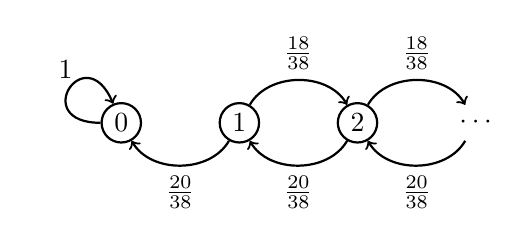
\begin{tikzpicture}
      \tikzset{punkt/.style={circle, thick, draw=black, minimum width=0.5cm,inner sep=0}}
      \node[punkt] at (-2.5, 0)      (a){$0$};
      \node[punkt] at (-1, 0)  (b){$1$};
      \node[punkt] at (0.5, 0)    (c){$2$};
      \tikzset{markus_m/.style={circle, thick, draw=white, minimum width=0.5cm,inner sep=0}}
      \node[markus_m] at (2, 0)    (d){$\cdots$};

      \draw[->, thick] (a) edge[out= 180, in = 113, looseness=8] node[above]{$1\;$} (a);
      \draw[->, thick] (b) edge[bend left=60] node[below]{$\frac{20}{38}$} (a);
      \draw[->, thick] (b) edge[bend left=60] node[above]{$\frac{18}{38}$} (c);
      \draw[->, thick] (c) edge[bend left=60] node[below]{$\frac{20}{38}$} (b);
      \draw[->, thick] (c) edge[bend left=60] node[above]{$\frac{18}{38}$} (d);
      \draw[->, thick] (d) edge[bend left=60] node[below]{$\frac{20}{38}$} (c);
    \end{tikzpicture}
    \caption{Overgangsgrafen for spillet roulette.}
    \label{fig:transpositions_graf_roullete}
  \end{figure}\noindent
  Bemærk, at da $X$ har et uendeligt udfaldsrum, har overgangsgrafen også uendeligt mange knudepunkter.
\end{example}

Vi vil nu introducere følgende sætning, som giver os mulighed for at beregne $n$ skrids overgangsmatricer.
\begin{thm} \label{thm:n_skrids_transpositions_matrix}
Lad $\{X_n\}_{n \geq 0}$ være en Markov kæde, så er $P_X(n) = P_X^n$ for $n \in \N$.
\end{thm}
\begin{proof}
Vi beviser dette ved induktion. For $n = 1$ gælder ligheden per definition. Antag nu, at $P_X(n - 1) = P_X^{n - 1} = [p_{ij}(n - 1)]$, så er 
\begin{align*} 
    p_{ij}(n) = P(X_n = j \;| X_0 = i) &\stackrel{(a)}= \sum_{k \in S} P(X_n = j\; | X_{n - 1} = k, X_0 = i) P(X_{n - 1} = k\; | X_0 = i) \\
    &\stackrel{(b)}= \sum_{k \in S} P(X_n = j\; | X_{n - 1} = k) P(X_{n - 1} = k\; | X_0 = i) \\
    &= \sum_{k \in S} p_{jk}p_{ki}(n - 1) 
\end{align*}
Hvor lighed $(a)$ følger af sætning \ref{thm:LPT}, $(b)$ af Markov betingelsen. Men $\displaystyle \sum_{k \in S} p_{jk}p_{ki}(n - 1)$ er blot indgang $(i, j)$ i matrix produktet $P_X P_X(n - 1) = P_X P_X^{n - 1} = P_X^n$, per vores induktions antagelse.
\end{proof}

\begin{defn}
  Lad $\{X_{n}\}_{n \geq 0}$ være en Markov kæde, og lad $i \in S$:
  \begin{enumerate}[i)]
    \item Hvis $P(X_{n} = i \text{ for et } n \in \N \;| X_{0} = i) = 1$ kaldes $i$ \textbf{rekurrent}.
    \item Hvis $P(X_{1} = i \;| X_{0} = i) = 1$, så kaldes udfaldet $i$ for \textbf{absorberende}.
    \item Hivs $P(X_n = i \text{ for et } n \in \N \;| X_0 = i) < 1$ kaldes udfaldet \textbf{transient}
  \end{enumerate}
\end{defn}

\begin{remark}
  Det noteres, at ethvert absorberende udfald også er et eksempel på et rekurrent udfald.
\end{remark}

\begin{example}
  Betragt igen spillet roulette og overgangsgrafen i figur \ref{fig:transpositions_graf_roullete} samt overgangsmatricen fra \ref{eq:transpositions_graf_roullete}. Det noteres, at udfaldet $0$ er et eksempel på et absorberende og rekurrent udfald, da $P(X_{1} = 0 | X_{0} = 0) = 1$. Derudover bemærkes det, at alle $i \in S \backslash \{0\}$ er eksempler på ikke rekurrente udfald, da $\exists n \in \N: P(X_{n} = 0 | X_{0} = i) > 0$. Tilgengæld er alle udfald $i \neq 0$ transiente, da $p_{ii}(2) = \sum_{j=0}^{\infty} p_{ij}p_{ji} > 0$, jævnfør sætning \ref{thm:n_skrids_transpositions_matrix}.
\end{example}

\begin{defn}
Lad $\{X_n\}_{n \geq 0}$ være en Markov kæde og $i, j \in S$. Udfaldene $i$ og $j$ siges, at \textbf{kommunikere}, skrevet $i \to j$, hvis $\exists m \in \N_0$, således $p_{ij}(m) > 0$. Hvis $i \to j$ og $j \to i$ siges $i$ og $j$ at \textbf{intrakommunikere}, skrives $i \leftrightarrow j$.\\ Lad $C \subseteq S$.
\begin{enumerate}[i)]
    \item Så kaldes $C$ \textbf{lukket} hvis $p_{ij} = 0$ for alle $i \in C, j \not \in C$. 
    \item og hvis  $i \leftrightarrow j$ for alle $i, j \in C$ kaldes $C$ \textbf{irreducibel}.
\end{enumerate}
\end{defn}

\begin{defn}
Lad $\{X_n\}_{n \geq 0}$ være en Markov kæde. En vektor $\bs{\pi}$, med indgange $\pi_j \in [0,1]$ for $j \in S$, kaldes en \textbf{stationær fordeling} af $\{X_n\}_{n \geq 0}$, hvis $\bs{\pi}P_X = \bs{\pi}$ og $\displaystyle \sum_{j \in S} \pi_j = 1$.
\end{defn}
Fordelingen kaldes stationær fordi $\bs{\pi} P_X^n = \bs{\pi} P_X^{n - 1} = \cdots = \bs{\pi} P_X = \bs{\pi}$.
% Yay endeligt et nyt eksempel
\begin{example}
  Et firma laver ventiler, hvis ventil $X_{n}$ virker gør ventil $X_{n + 1}$ det også med sandsynlighed $0.9$, og hvis ventil $X_{n}$ ikke virker, virker ventil $X_{n + 1}$ heller ikke med sandsnynlighed $0.6$. Vi lader $X_{n} = 1$, hvis ventilen virker, og $X_{n} = 0$ ellers. Overgangsgrafen for Markov kæden kan ses på figure \ref{fig:eksempel_stationary}
  \begin{figure}[H]
    \centering
    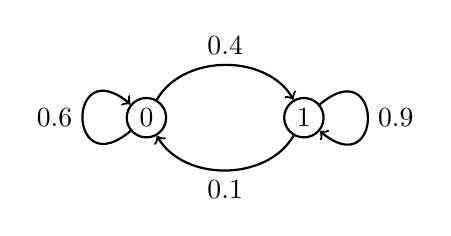
\begin{tikzpicture}
      \tikzset{punkt/.style={circle, thick, draw=black, minimum width=0.5cm,inner sep=0}}
      \node[punkt] at (1, 0)  (a){$1$};
      \node[punkt] at (-1, 0) (b){$0$};

      \draw[->, thick] (a) edge[out= 40, in = 320, looseness=8] node[right]{$0.9$} (a);
      \draw[->, thick] (b) edge[bend left=60] node[above]{$0.4$} (a);
      \draw[->, thick] (b) edge[out= 220, in = 140, looseness=8] node[left]{$0.6$} (b);
      \draw[->, thick] (a) edge[bend left=60] node[below]{$0.1$} (b);
    \end{tikzpicture}
    \caption{Overgangsgraf for processen}
    \label{fig:eksempel_stationary}
  \end{figure}\noindent
  Fra overgangsgrafen ses det, at alle udfald intra kommunikere, og Markov kæden derfor er et eksempel på en irreducibel Markov kæde. Vi ser derudover, at ligningen
  \begin{equation*}
    \pi P_{X} = \pi \begin{bmatrix}
                      0.6 & 0.4 \\ 0.1 & 0.9
                    \end{bmatrix} = \pi
  \end{equation*}
  løses af $\pi = s \begin{bmatrix} 1 & 4 \end{bmatrix}$, hvor $s \in \R$.
  Men vi har derudover at $\pi_{1} + \pi_{2} = 1$, samt $\pi_{1}, \pi_{2} \geq 0$, da der er tale om en fordeling.
  Det følger derfor at $\pi = \begin{bmatrix} 0.2 & 0.8 \end{bmatrix}$.
\end{example}

\chapter{Forgreningsprocesser}
%En stokastisk proces i det diskrete tilfælde er en samling af diskrete stokastiske variabler, der har værdier i en mængde, som kaldes \textbf{tilstandsrum}. Mængden er indekseret af \textbf{indeksmængden}, hvor det er typisk de naturlig tal, der anvendes. 
Dette afsnit bygger på \cite{sandsynlighedsBog} og \cite{grimsandsynlighedsBog}.
Et eksempel på en stokastisk proces er den såkaldte forgrenings process, som modellere et ``et-kønnet'' stamtræ, teorien stammer oprindeligt England, hvor Francis Galton, ønskede at undsøge hvilke efternavne, som ville uddø. Processen kan bruges til at modellere mange forskellige stokastiske phenomener, eksempelvis virus, jordskælv og fission.
Lad de diskret stokastiske variable $X_{n,k}$ betegne antallet af \textbf{afkom} den $k$'te forfader i den $n$'te \textbf{generation} får og lad dem være iid med pmf $p_X$. Den første forfader $Z_0$ kaldes \textbf{stamforfaderen}.
Størrelsen på hver generation, betegnet $Z_n$, danner en følge, som kaldes en stokastisk forgreningsproces eller en Galton-Watson proces.
\begin{defn}\label{def:forgreningsproces}
Lad $X_{n,k}$ være iid diskret stokastiske variable med udfaldsrum i $\N_0$ og pmf $p_X$. En \textbf{forgreningsproces} er en følge $\{Z_n\}_{n\geq 0}$ beskrevet ved følgende induktion
\begin{align*}
    Z_n=\begin{cases}
        1&n=0\\
        \sum_{k=1}^{Z_{n-1}}X_{n,k}&n>0,Z_{n-1}>0\\
        0&n>0,Z_{n-1}=0
        \end{cases}
\end{align*}
Fordelingen givet ved $p_X$ kaldes for \textbf{afkomsfordelingen}.
\end{defn}

Et eksempel på en forgeningsproces kan ses i figur \ref{fig:eksforgreningsproces}, som viser et stamtræ for en slægt, hvor stamforfaderen fik to børn $A$ og $B$, som videre fik deres egen slægt $A$ og $B$.

\begin{figure}[H] 
 \centering
    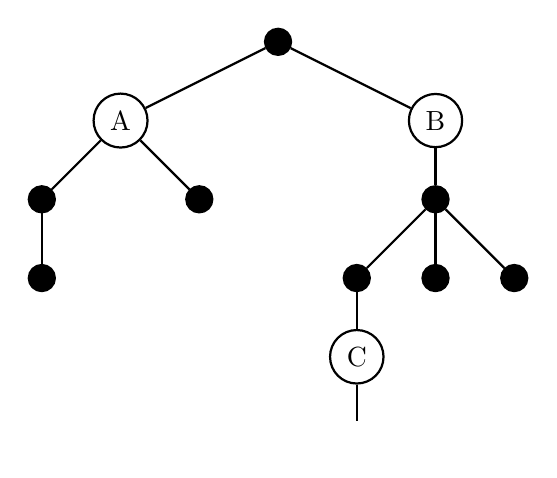
\begin{tikzpicture}
    \tikzset{punkt/.style={circle,thick, draw=black, minimum width=0.1cm,fill=black}}
    \tikzset{punkd/.style={circle,thick, draw=white, minimum width=0.1cm,fill=white}}
    \tikzset{punkta/.style={circle,thick, draw=black, minimum width=0.1cm}}

%Z_0
    \node[punkt] at (0.0, 3.0) (z_1) {};
    
    
%Z_1    
    \node[punkta] at (-2.0, 2.0) (z_21) {A};
    \node[punkta] at (2.0, 2.0) (z_22) {B};
    \draw [-, thick, draw=black] (z_1) -- (z_21);
    \draw [-, thick, draw=black] (z_1) -- (z_22);
%Z_2
    \node[punkt] at (-1.0, 1.0) (z_312) {};
    \node[punkt] at (-3.0, 1.0) (z_311) {};
    \draw [-, thick, draw=black] (z_21) -- (z_312);
    \draw [-, thick, draw=black] (z_21) -- (z_311);
    
    \node[punkt] at (2.0, 1.0) (z_321) {};
    \draw [-, thick, draw=black] (z_22) -- (z_321);
%Z_3
    \node[punkt] at (-3.0, 0.0) (z_411) {};
    \draw [-, thick, draw=black] (z_311) -- (z_411);
    
    \node[punkt] at (3.0, 0.0) (z_413) {};
    \node[punkt] at (2.0, 0.0) (z_412) {};
    \node[punkt] at (1.0, 0.0) (z_411) {};
    \draw [-, thick, draw=black] (z_321) -- (z_413);
    \draw [-, thick, draw=black] (z_321) -- (z_412);
    \draw [-, thick, draw=black] (z_321) -- (z_411);
%Z_4
    \node[punkta] at (1.0, -1.0) (z_511) {C};
    \draw [-, thick, draw=black] (z_411) -- (z_511);

    \node[punkd] at (1.0, -2.0) (z_611) {};
    \draw [-, thick, draw=black] (z_511) -- (z_611);
    
    \end{tikzpicture}
  \caption{En forgreningsproces, hvor $Z_0=1, Z_1=2, Z_2=3, Z_3=4$, $Z_4=1$}
  \label{fig:eksforgreningsproces}
\end{figure}
Et yderligere begreb omkring generationer \textbf{familie}, hvilket er mængden af afkom i generation $(n+1)$ hvert afkom fra genreationen $(n)$ får. Denne mængde kan er selvfølglig tom, hvis afkommet ingen afkom før. I eksempelet er $A$ og $B$ en familie, da de er de to afkom af $Z_0$. Yderligere bliver $Z_1$ der dannet $2$ familier, $Z_2$ danner også $2$ familier, og $Z_3$ danner $1$.

\begin{prop}\label{prop:pgfforgreningsproces}
Lad $\{Z_n\}_{n\geq 0}$ være en forgreningsproces og lad $G$ være pgf til afkomstfordelingen. Da er pgf'er $G_n$ for $Z_n$ givet ved
\begin{align*}
    G_n(s)=
    \begin{cases}
        s & n=0\\
        G_{n-1}(G(s)) & n>0
    \end{cases}
\end{align*}
\end{prop}
\begin{proof}
Det vides, at $Z_0\equiv 1$, altså har $Z_0$ kun et udfald.
Det eneste ikke-nul led i summen fra definitionen af pgf \ref{pgf} bliver da $k=1$, hvilket giver at $G_0(s)=s$.\\
%For $Z_1$ gælder det at $Z_1=\sum_{k=1}^{Z_0}X_{1,k}=X_{1,1}$, altså har $Z_1$ pgf $G$.
For $n>0$ anvendes Galton-Watson formlen fra proposition \ref{prop 3.39} direkte med $N = Z_{n - 1}$.
\end{proof}
\begin{rem}
    Det gælder for notation for pgf'er, at $G=G_1$
\end{rem}
Det kan være interessant at undersøge om en slægt vil uddø på et tidspunkt, og denne hændelse defineres på en følgende måde. 
\begin{defn}%Extinction
    Lad $\{Z_n\}_{n\geq 0}$ være en forgreningsproces.
    Hændelsen, hvor forgreningsprocessen uddør, noteres $\Omega$ og defineres som
    \begin{align*}
        \Omega = \bigcup_{n=0}^\infty\{Z_n=0\}
    \end{align*}
\end{defn}

I figur \ref{fig:eksforgreningsproces}, uddør barn $A$'s slægt i generation $Z_4$, mens nogle af barn $B$'s børnebørn ikke får afkom og deres slægter uddør, dog fortsætter slægt $B$ igennem $C$'s slægt.

\begin{lem}
    Lad $\{Z_n\}_{n\geq 0}$ være en forgreningsproces. Så gælder det, at
    \begin{align*}
        \Omega = \left\{\lim_{n\rightarrow\infty}Z_n = 0\right\}
    \end{align*}
\end{lem}
\begin{proof}
    Fra definition \ref{def:forgreningsproces} ses, at $Z_n=0\implies Z_{n+1}=0$, hvilket giver $\{Z_n=0\}\subseteq\{Z_{n+1}=0\}$. Ved induktion ses det herfra, at
    \begin{align*}
        \forall k\geq 0:\bigcup_{n=0}^k\{Z_n=0\}=\{Z_{k}=0\}
    \end{align*}
    Lader vi $k\rightarrow\infty$ opnås det ønskede resultat
    \begin{align*}
        \Omega=\bigcup_{n=0}^\infty\{Z_n=0\}=\left\{\lim_{n\rightarrow\infty}Z_n = 0\right\}
    \end{align*}
\end{proof}

Sandsynligheden for at forgreningsprocessen uddør er givet som grænseværdien af pgf'ernes værdier i $0$.
\begin{prop}
Lad $\{Z_n\}_{n \geq 0}$ være en forgreningsproces og lad $Z_n$ have pgf $G_n$. Sandsynligheden for, at forgreningsprocessen uddør, er givet ved
\begin{align*}
    P(\Omega)=\lim_{n\rightarrow\infty}G_n(0)
\end{align*}
\end{prop}
\begin{proof}
\begin{align*}
    P(\Omega)&=P\left(\lim_{n\rightarrow\infty}Z_n = 0\right)\\
    &=\lim_{n\rightarrow\infty}P(Z_n = 0)\\
    &=\lim_{n\rightarrow\infty}G_n(0)
\end{align*}
jævnfør proposition \ref{prop:pgfI0Og1}.
\end{proof}

En hurtig måde til at finde sandsynligheden for, at forgreningen uddør er at kigge på fikspunktet $s=G(s)$  
\begin{prop} \label{prop:prop8.7}%8.7
Lad afkomsfordelingen af en forgreningsproces have pgf $G$. Så er den mindste løsning til $s=G(s)$ i intervallet $s\in[0,1]$ givet ved $\eta=P(\Omega)$.
\end{prop}
\begin{proof}
Først vises det at $\eta$ er en løsning, hvorefter det vises at det er den mindste løsning.
Lad $X$ være antallet af afkom stamforfaderen får.
Hvis $X=k$, så eksisterer der $k$ uafhængige forgreningsprocesser, der skal uddø, for at slægten uddør.
Sandsynligheden, for at dette sker, er $\eta^k$, da forgreningsprocesserne er uafhængige af hinanden.
Dette giver, at 
\begin{align*}
    \eta=\sum_{k=0}^{\infty}P(\Omega|X=k)P(X=k)=\sum_{k=0}^{\infty}q^kP(X=k)=G(q)
\end{align*}
jævnfør sætning \ref{thm:LTP} og det ses, at $P(\Omega)=\eta$ løser $s=G(s)$.\\ 
Antag nu at der er en anden løsning $r\in[0,1]$.
Fra proposition \ref{prop:pgfforgreningsproces} har vi at
\begin{align*}
    r=G_0(r)=G_0(G(r))=G_1(r)=\dots=\lim_{n\to\infty}G_n(r)
\end{align*}
Da pgf'er er voksende jævnfør korollar \ref{cor:egenskaberVedPGF}, og $r\geq 0$, så er
\begin{align*}
    r = \lim_{n\to\infty}G_n(r) \geq \lim_{n\to\infty}G_n(0)=P(\Omega)=\eta
\end{align*}
og hermed er $\eta$ den mindste løsning til $s=G(s)$.
\end{proof}

Den forventede værdi af afkom kan benyttes til at undersøge sandsynligheden for at slægten uddør.
\begin{prop} \label{prop:prop8.9}%8.9
  Lad en forgreningsproces $\{Z_{n}\}_{n \geq 0}$ have en forventede værdi $\mu$ af afkomsfordelingen, $p_{X}$. Hvis $\mu > 1$, så er $P(\Omega) < 1$, ellers hvis $\mu \leq 1$ og $p_{X}(0) > 0$, så er $P(\Omega) = 1$.
\end{prop}
\begin{proof}
  Det vides at $G_{X}$ er en voksende og konveks funktion jævnfør korollar \ref{problem133}.
  Antag $\mu \leq 1$ og $p_{X}(0) > 0$, så er $G_{X}$ voksende fra $G_{X}(0) = p_{X}(0) > 0$ til $G(1) = 1$, jævnfør proposition \ref{prop:pgfI0Og1}. Dette medfører at den mindste løsning til $s = G_{X}(s)$, givet ved $s = 1$, heraf følger det at $P(\Omega) = 1$, jævnfør proposition \ref{prop:prop8.7}.
  Antag nu at $\mu > 1$, så må $G_{X}(s)$ krydse linjen $y = s$, da $G_{X}'(1) = \mu > 1$, jævnfør \ref{prop 3.37} og $G_{X}$ er voksende. Altså eksistere $s < 1$ således $s = G_{X}(s)$, heraf følger det at $P(\Omega) = s$, jævnfør proposition \ref{prop:prop8.7}.
\end{proof}

%\begin{proof} % GAMELT BEVIS
%    Fra proposition \ref{prop 3.37} gælder det, at $\mu=G'(1)$. Hvis $p_X(0)=0$, så er $\mu > 1$, såfremt $\exists n \in \N, n > 1: p_{X}(n) > 0$ og $P(\Omega)=0$. Bemærk at beviset for specialtilfældet, hvor $G'(s)\equiv 1$ er undladt.
%    \\
%    Hvis $p_{X}(0) = 1$
%    \quad Antag nu at $1 > p_X(0) >0$. Fra korollar \ref{problem133} vides det, at pgf'en $G(s)$ er konveks og voksende. Yderligere så er pgf'en stigende fra $G(0)=p_X(0)>0$ til $G(1)=1$. Hvis $\mu>1$, så må $G(s)$ krydse linjen $y=s$, samt er den første skæringen sandsynligheden, for at slægten uddør, hvilket er skarpt mindre end $1$ jævnfør proposition \ref{prop:prop8.7}.
%    Hvis i stedet $\mu\leq1$, så er der ingen skæring med $y=s$ før $1$, og hermed er sandsynligheden $1$.
%\end{proof}
Figur \ref{fig:proofprop8.9} illustrerer de forskellige tilfælde i proposition \ref{prop:prop8.9}. Den blå graf er $\mu\leq1$, den røde graf er $G(0)=0$, den grønne graf er $\mu>1$, og så er den sorte graf $y=s$. 
\begin{figure}[H]
    \centering
   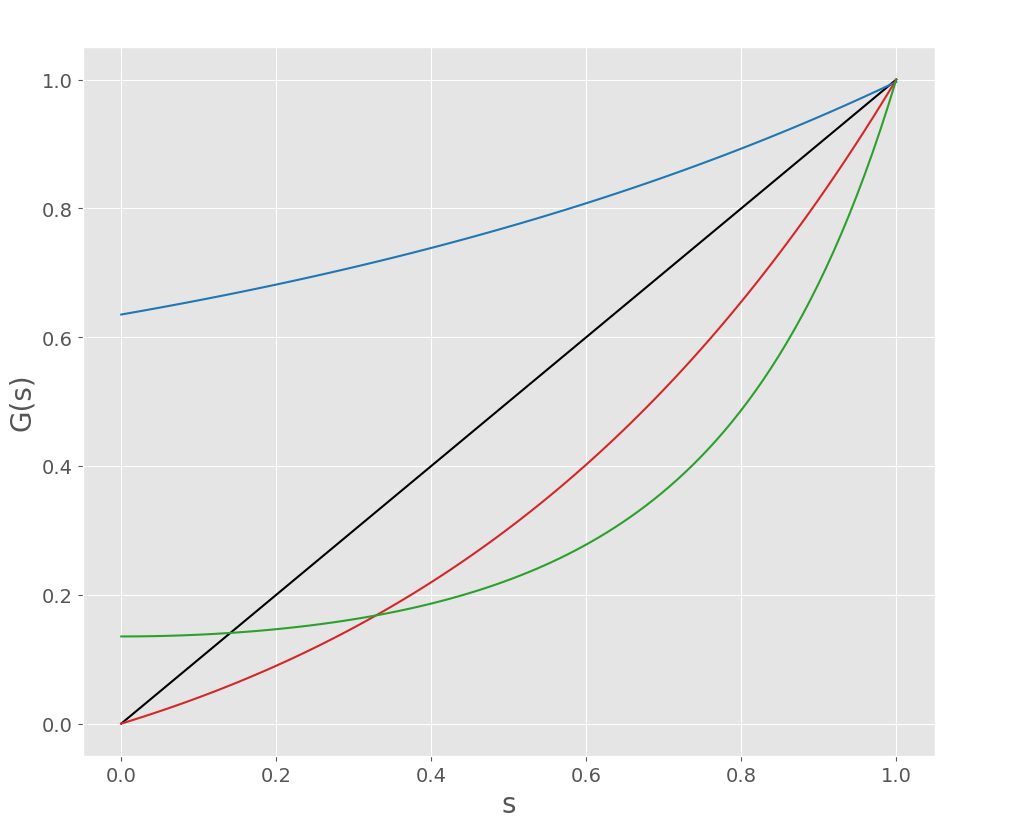
\includegraphics[scale=0.5]{fig/img/Markus.png}
    \caption{Forskellige pgf'er og linjen $y = s$, markeret med sort}
    \label{fig:proofprop8.9}
\end{figure}

\begin{exmp} %Ins fra 8.18
    Betragt en slægt hvor afkomsfordelingen har følgende pmf
    \begin{align*}
        p_X(k) = \begin{cases}
                    3/4  & \text{for } k = 0 \\
                    1/8  & \text{for } k = 1 \\
                    1/8  & \text{for } k = 2 \\
                    0 & \text{ ellers}
                \end{cases}
    \end{align*}
Vi har, at 
\begin{align*}
    G(s)=\frac{3}{4}+\frac{1}{8}s+\frac{1}{8}s^2
\end{align*}
% hvor $G(0)=\frac{3}{4}$. Videre har vi, at
% \begin{align*}
%     G_2(s)=G(G(s))=\frac{3}{4}+\frac{1}{8}\left(\frac{3}{4}+\frac{1}{8}s+\frac{1}{8}s^2\right)+\frac{1}{8}\left(\frac{3}{4}+\frac{1}{8}s+\frac{1}{8}s^2\right)^2
% \end{align*}
% hvor 
% \begin{align*}
%  G_2(0)=\frac{3}{4}+\frac{1}{8}\left(\frac{3}{4}\right)+\frac{1}{8}\left(\frac{3}{4}\right)^2=\frac{3}{4}+\frac{3}{32}+\frac{9}{128}=\frac{117}{128}\approx 0,844   
% \end{align*}
% Hvis dette fortsættes fåes $G_3(0)\approx0.969$, $G_4(0)\approx0.989$, $G_5(0)\approx0.996$, og $G_6(0)\approx0.998$. Hermed vil $P(\Omega)=\lim_{n\to\infty}=1$. 

Fra proposition \ref{prop:prop8.7} vides, at den mindste løsning til $s=G(s)$ er $P(\Omega)$.
\begin{align*}
    s=\frac{3}{4}+\frac{1}{8}s+\frac{1}{8}s^2
\end{align*}
hvor løsningerne til andengradsligningen er $1$ og $6$, hvor $P(\Omega)=1$ så er den mindste løsning til ligningen. 

En anden måde, resultatet kan findes, er ud fra proposition \ref{prop:prop8.9}, da $G'(s)=\frac{1}{8}+2\frac{1}{8}s$, så 
\begin{align*}
    G'(1)=\mu=\frac{1}{8}+2\frac{1}{8}=0.375
\end{align*}
hvilket er mindre end $1$, og hermed er $P(\Omega)=1$
\end{exmp}


\begin{prop} %8.8 
    Lad $\mu=E[X]$ og $\sigma^2=\Var[X]$, så så er $E[Z_n]=\mu^n$ og
    \begin{equation*}
        \Var[Z_n] = \begin{cases} 
        n\sigma^2 & \text{ hvis } \mu =1\\
        \dfrac{\sigma^2(\mu^n-1)\mu^{n-1}}{\mu-1} & \text{ hvis } \mu \neq 1
        \end{cases}
    \end{equation*} 
\end{prop}

\begin{proof}
Ved at benytte proposition \ref{prop:cor 3.13} fåes det, at $E[Z_N]=\mu E[Z_{n - 1}]$, heraf fåes
\begin{align*}
    E[Z_n]=\mu E[Z_{n - 1}]=\mu^2E[Z_{n-2}]= \dots = \mu^{n - 1} E[Z_1] = \mu^n
\end{align*}
Vi beviser formlerne for varians ved hjælp af induktion. 
Det gælder, at $\Var[Z_1] = \Var[X] = \sigma^2$, da der kun er et individ til at reproducere.
Benyt proposition \ref{prop:cor 3.13} med $N = Z_{n- 1}$ til at skrive
\begin{align*}
    \Var[Z_n] = E[Z_{n - 1}]\Var[X] + E[X]^2\Var[Z_{n - 1}]  = \mu^{n - 1}\sigma^2 + \mu^2\Var[Z_{n - 1}]
\end{align*}
Antag at $\mu = 1$ og formelen gælder for $\Var[Z_{n - 1}]$, vi har derfor, at 
\begin{equation*}
 \Var[Z_n] = 1^{n-1}\sigma^2 + 1^2 (n - 1)\sigma^2 = n \sigma^2   
\end{equation*}
per vores induktions antagelse.
Antag nu, at $E[X] = \mu \neq 1$, igen har vi, at formelen gælder for $\Var[Z_1]$, da 
\begin{equation*}
    \frac{\sigma^2(\mu - 1)\mu^0}{\mu - 1} = \sigma^2 = \Var[Z_1]
\end{equation*}
Antag derfor, at resultatet gælder for $\Var[Z_{n - 1}]$, så følger det, at
\begin{align*}
    \Var[Z_n] &= \mu^{n - 1} \sigma^2 + \mu^2 \frac{\sigma^2(\mu^{n  - 1} -1)\mu^{n-2}}{\mu-1} \\
    &= \frac{\sigma^2\mu^{n - 1}(\mu - 1)}{\mu - 1} + \frac{\sigma^2(\mu^{n - 1}-1)\mu^{n}}{\mu-1} \\
    &= \sigma^2\frac{\mu^{n - 1}(\mu - 1) + \mu^{n - 2}(\mu^{n - 1} - 1)}{\mu - 1}
    = \sigma^2 \frac{-\mu^{n - 1} + \mu^{2n - 1}}{\mu - 1} = \frac{\sigma^2(\mu^n - 1)\mu^{n - 1}}{\mu - 1}
\end{align*}
hvilket afslutter induktionsskridtet og beviset.
\end{proof}
Vi vil nu undersøge om antallet af individer kan gå imod et $n \in \N$.

\begin{prop} %8.10 (vi mangler bemærkningen under)
Hvis $P(Z_n \to 0) = \eta$ for $n \to \infty$, så gælder det, at  $P(Z_n \to \infty) = 1 - \eta$ for $n \to \infty$.
\end{prop}
\begin{proof}
Antag først at $Z_n\not\to\infty$.
Dette betyder, at følgen har en øvre grænse $M$, således at $Z_n \leq M \; \forall n\in \N$.
Generation $Z_{n+1}=0$, hvis ingen individer i forrige generation får afkom, hvilket har sandsynlighed $p_X(0)^{Z_n}\geq p_X(0)^{M}>0$.
Da denne sandsynlighed er positiv for alle $Z_n$, må der efter nok generationer være en generation hvor $Z_n=0$.
Altså gælder det for $n \to \infty$, at $Z_n\not\to\infty\implies Z_n\to0$.
Det gælder også, at $Z_n\to0\implies Z_n\not\to\infty$, så hændelserne er ækvivalente. Med dette konkluderes, at $P(Z_n \to 0) = P(Z_n\not\to\infty) = \eta \implies P(Z_n\to\infty) = 1-\eta$ for $n \to \infty$.
\end{proof}

\subsection{Revisted (skal ikke være her, men så har vi har styr på hvad der igang)}
Gej
Der er en række eksempler som kan være besværlige at håndtere med de indtil videre præsenterede værktøjer.
Eksempelvis hvis $Z_0=1$, men hvor der for hver familie gælder, at   
\begin{align*}
P(Z_1=0)<0    
\end{align*}
så er $0$ i en absorberende tilstand, og alle andre tilstand er transiente. Derfor er hele hele kæden ikkereducerbar, men  %rekurrent skal indskrives 
 når familien er $0$, så er den. Så gælder det, at $P(Z_1=0)=1$. Dog eksisterer der en stationær fordeling 
\begin{align*}
    \bs{\pi}=\begin{bmatrix}
1\\
0\\
0\\
\vdots\\
0
\end{bmatrix}
\end{align*}
da $\pi_0$ i sig selv er irreducibel.  

Dette fortæller også dog ikke noget om processen. En måde at gå til dette problem er, at kigge på opførelsen af processen ved visse hændelser med visse betingelser. 

I den resterende del af afsnittet arbejdes der med dette problem. Vi har hermed nogen faste antagelse og notationer. Der kigges på en familie af størrelse $Z_1$ med pgf og pmf 
\begin{align*}
    G(s)=E[s^{Z_1}] \quad f(k)=P(Z_1=k)
\end{align*} 
Lad generation for forgreningens død være noteret $T=\inf{n:Z_n=0}$, samt  
lad $E_n={n<T<\infty}$
være hændelserne, hvor forgreningen uddør efter. 

Vi antager også for pmf'en, at $0<f(0)+f(1)<1$ og $0<f(0)$, hvilket medfører, at 
\begin{align*}
    0<P(E_n)<1    
\end{align*}
gælder for sandsyndligen af $E_n$. Det gælder også, at $0< P(\Omega)\leq 1$

Fordelingen for $Z_n$ undersøges under betingelsen af forekomsten af $E_n$. Lad den betinget sandsynlighed af hændelsen $Z_n=j$ og $E_n$ være givet ved 
\begin{align*}
    p_j(n)=P(Z_n=j | E_n)
\end{align*}
så er grænseværdien 
\begin{align*}
q_j=\lim_{n\to \infty} p_j(n)    
\end{align*}
interessant, hvis den eksisterer, hvilket ses i følgende lemma. 

\begin{lem}
Hvis $E[X] < \infty$, så eksistere grænseværdien $\lim_{n \to \infty} p_j (n) = {}_0\pi_j$. Derudover overholdet den genererende funktion
\begin{equation*}
    G^\pi(s) = \sum_j {}_0 \pi_j s^j
\end{equation*}
ligningen 
\begin{equation} \label{alg:alg6.7.2grim}
    G^\pi\left(\frac{G_X(s\eta)}{\eta}\right) = m G^\pi(s) + 1 - m
\end{equation}
hvor $\eta = P(\Omega)$ og $m = G'(\eta)$.
\end{lem}
\begin{proof}
For $s \in [0, 1)$, lad
\begin{align*}
    G_n^\pi (s) = E(s^{Z_n} | E_n) = \sum_j {}_0p_j(n)s^j &\stackrel{(a)}= \sum_j s^j \frac{P(Z_n = j, E_n))}{P(E_n)} \\ 
    &\stackrel{(b)} = \frac{1}{\eta - G_n(0)} \sum_j s^j P(Z_n = j, E_n) \stackrel{(c)} = \frac{G_n(s\eta) - G_n(0)}{\eta - G_n(0)}
\end{align*}
hvor $G_n(s) = E(s^{Z_n})$. Lighed $(a)$ følger af ${}_0p_j(n) = \dfrac{P(Z_n = j, E_n)}{P(E_n)}$ per definition. Lighed $(b)$ af det faktum at $P(E_n) = P(\{n < T < \infty\}) = P(T < \infty) - P(T \leq n) = \eta - G_n(0)$, da $G_n(0) = P(Z_n = 0)$, og $(c)$ følger af
\begin{align*}
    P(Z_n = j, E_n) &= P(Z_n = j \text{ og alle børnenes slægter uddør }) \\
    &= P(Z_n = j) \eta^j, \text{ hvis } j \geq 1,
\end{align*}
Definer nu funktionerne 
\begin{equation*}
    H_n(s) = \frac{\eta - G_n(s)}{\eta - G_n(0)}, \quad h(s) = \frac{\eta - G(s)}{\eta - s}, \quad 0 \leq s \leq \eta
\end{equation*}
det noteres at 
\begin{equation*} \label{eq:lemmaErAids}
    1 - H_n(s \eta) = 1 - \frac{\eta - G_n(s\eta)}{\eta - G_n(0)} = \frac{\eta - G_n(0) - \eta + G_n(s\eta)}{\eta - G_n(0)} = G_n^\pi(s)
\end{equation*}
% NOTE: Hvorfor er det her vigtigt
Eftersom at $H_n$ har værdi mængde $[0, \eta)$ og $G_n^\pi$ har værdi mængde $[0, 1)$, så gælder det at 
\begin{align*}
    \frac{h(G_{n - 1}(s))}{h(G_{n - 1}(0)} \stackrel{(a)}=
    \frac{\dfrac{\eta - G_{n}(s)}{\eta - G_{n - 1}(s)}}{\dfrac{\eta - G_{n}(0)}{\eta - G_{n - 1}(0)}} &= 
    \frac{\eta - G_{n}(s)}{\eta - G_{n - 1}(s)}\frac{\eta - G_{n-1}(0)}{\eta - G_{n}(0)} \\
    &= 
    \frac{(\eta - G_{n}(s))(\eta -  G_{n - 1}(0))}{(\eta - G_n(0)(\eta - G_{n - 1}(s))}
    =
    H_n(s)H_{n - 1}(s)^{-1}
\end{align*}
hvor $(a)$ følger af proposition \ref{prop:pgfforgreningsproces}. 

Det gælder at $h$ er voksende da $G$ er konveks på $[0, \eta)$ jævnfør korollar \ref{cor:egenskaberVedPGF}, hvilket medfører er $G(s) \leq s$. Det gælder derudover per samme korollar at $G_{n - 1}$ er voksende. Hvilket giver os $H_n(s) \geq H_{n - 1}(s)$ for $s < \eta$. Derfor gælder det at grænsenværdien 
\begin{equation*}
    \lim_{n \to \infty} H_n(s\eta) = H(s\eta)
\end{equation*}
eksistere, da $H_n(s) > 0 \forall n \in N, s \in [0, \eta)$ og denne grænseværdi giver os sammen med ligning \ref{eq:lemmaErAids}, os grænseværdien at grænseværdien
\begin{equation*}
    \lim_{n \to \infty} G_n^\pi(s) = G^\pi(s)
\end{equation*}
også eksistere, for $s \in [0, 1)$. Ved at tage grænseværdien i ligning \eqref{eq:lemmaErAids} opnåes
\begin{equation}\label{alg:alg4bevislemma6.7.1grim}
   G^\pi(s) = 1 - H(s \eta), \text{ hvis } s \in [0, 1) 
\end{equation}
\textbf{Grimmit skriver at dette giver os eksistensen af ${}_0\pi_j$, men følger det ikke af at $G^\pi(s)$ eksistrere som grænse værdien til $G^\pi_n(s)$?} 

Det gælder derudover at hvis $s \in [0, \eta)$ er 
\begin{equation*}\label{eq:HnGs}
    H_n(G(s)) = \frac{\eta - G_n(G(s))}{\eta - G_n(0)} = \frac{\eta - G(G_n(0))}{\eta - G_n(0)} \cdot \frac{\eta - G_{n + 1}(s)}{\eta - G_{n + 1}(0)} = h(G_n(0))H_{n + 1}(s)
\end{equation*}
da $G(G_n(0)) = G_{n + 1}(0)$.
Bemærk at når $n \to \infty$, går $G_n(0)$ imod $\eta$ fra venstre. hvilket giver os
\begin{equation*}
    h(G_n(0)) \to \lim_{s \to \eta^+} \frac{\eta - G(s)}{\eta - s} = G'(\eta) \text{ for } n \to \infty
\end{equation*}
da $\eta = G(\eta)$, jævnfør proposition \ref{prop:prop8.7}. Lad nu $n \to \infty$ i ligning \eqref{eq:HnGs} for at opnå
\begin{equation} \label{alg:alg6bevislemma6.7.1grim}
    H(G(s)) = G'(\eta)H(s), \text { hvis } s \in [0, \eta)
\end{equation}
Benyt ligning \ref{alg:alg4bevislemma6.7.1grim} til at opnå
\begin{equation*}
    G^\pi(\eta^{-1}G(s)) + 1
\end{equation*}
Tilsidst \textbf{todo med ligningen}
\end{proof}

\begin{rem}
Når $\mu=E[Z_1] \leq 1$, så er det sikkert, at forgreningen uddør ifølge proposition \ref{prop:prop8.9}, således er $P(\Omega)=1$, samt $G'(P(\Omega))=\mu$. Dette leder til, at \eqref{alg:alg6.7.2grim} kan reduceres til 
\begin{align*}
    G^\pi(G(s))=\mu (G^\pi(s)-\mu)+1
\end{align*}
\end{rem}
\begin{cor} \label{cor:cor6.7.7grim}
Lad $\mu=E[Z_1]$. Hvis 
\begin{itemize}
    \item $\mu \neq 1$, så er $\sum_{j=0}q_j=1$. 
    \item $\mu=1$, så er $q_j=0$ for alle $j$. 
\end{itemize}
\end{cor}
\begin{proof}
Bevis af $\mu=1$:\\
Vi har, at $G'(P(\Omega))=1$ hvis og kun hvis $\mu=1$ fra bemærkningen. Hermed kan \eqref{alg:alg6.7.2grim} omskrives til \begin{align*}
    G^\pi(G(s))=G^\pi(s)
\end{align*}
da $P(\Omega)=1$, når $\mu\leq1$. Fra proposition \ref{prop:prop8.7} har vi, at hvis $\mu > 1$, så er $G(s)>s$ for alle $s<1$. Og da $G^\pi(G(s)) =G^\pi(s)$, og følgen $\{G_n(0)\}_{n \geq 0}$ konvergere imod $1$, da $G(1) = 1$ og talfølgen er voksende, har vi at $G^\pi(s)=G^\pi(0)=0$ for alle $s<1$. 

Hermed er $G^\pi(s)=\sum_j q_j s^j =0$, hvilket medfører, at
\begin{align*}
    q_j=0 \quad \text{for alle j}
\end{align*}

Bevis af $\mu\neq1$:\\ 
Modsat første tilfælde, så gælder det, at $\mu\neq1$ hvis og kun hvis $G'(P(\Omega))\neq 1$. Lad $s\to P(\Omega)$ i \eqref{alg:alg6bevislemma6.7.1grim}, så fåes
Lad ${s_n}_{n \geq 0}$ være en følge som konvergere imod nede fra $\eta$, da $H_n(s_n)$ konvergere uniformt har vi

\begin{align*}
    \lim_{s\to \eta^-}H(s)= \lim_{n \to \infty} H_n(s_n) = \lim_{n \to \infty} \frac{\eta - G_n(s_n)}{\eta - G_n(0)} = 0
\end{align*}
eftersom $G_n(s_n) \to \eta$, når $n \to \infty$.

Derfor fåes det fra \eqref{alg:alg4bevislemma6.7.1grim}, at
\begin{align*}
    \lim_{s\to 1} G^\pi(s)=\lim_{s\to 1} 1-H(sP(\Omega))=1 
\end{align*}
da $\lim_{s\to 1} H(sP(\Omega))=0$. Hermed
er
\begin{align*}
    \lim_{s\to 1} G^\pi(s)=\lim_{s\to 1} \sum_j q_js_j =1
\end{align*}
hvor $\sum_j q_j=1$
\end{proof}

Det er svært at undersøge forgrenningsprocceserne, hvor $\mu=1$ og $j\leq 1$, da
\begin{align}
    P(Z_n=j)\to 0 \quad \text{ forgreningen uddør}
    \\
    P(Z_n=j |E_n) \to 0 \quad \text{da } Z_n\to\infty \text{ under betingelse af } E_n 
\end{align}
Lad nu $\sigma^2=\Var[Z_1]$ og  
\begin{align*}
Y_n=\frac{Z_n}{n\sigma^2}    
\end{align*}
Så er det muligt at vise fordelingen for $Y_n$ betinget af $E_n$ er konvergent, når $n\to\infty$.  

\begin{thm} \label{thm:thm6.7.8grim}
Hvis $\mu=E[Z_1]$ og $G''(1)<\infty$, så overholder $Y_n$, at
\begin{align*}
    \lim_{n\to\infty}P(Y_n\leq y|E_n) = 1-e^{-2y}
\end{align*}
\end{thm} 
\begin{proof}

\end{proof}










\chapter{Simulering}

Dette afsnit bygger på \cite{sandsynlighedsBog} og \cite{grimsandsynlighedsBog}.
\section{Markovs ulighed}
\begin{theorem}
Hvis $X$ er en tilfældig variable med en begrænset middelværdi, så gælder
\begin{align*}
    P(|X|\geq a) \leq \frac{E[|X|]}{a} \text{ for alle } a > 0
\end{align*}
\end{theorem}
\begin{proof}
Lad $A=\{|X|\geq a\}$, så fremstilles indikator funktionen af $A$ $|X|\geq aI_a$. Så tages den forventede værdi på begge sider, hvorefter man kan flytte $a$ uden for.
\begin{align*}
E[|X|]\geq E[aI_a] = a E[I_a]
\end{align*} 
Til sidst divideres der med $a$ på begge sider. Eftersom den forventede værdi af indikartor funktionen er $P(A)$, så indsættes dette og giver det ænskede resultat.
\begin{align*}
    \frac{E[|X|]}{a} \geq P(A)
\end{align*} 
\end{proof}
Det er værd at bemærke at hvis $a<0$ så skal relationen vendes om.

\section{Chebyshews ulighed}
Chebyshews ulighed siger noget om hvad sansyndligheden er for at en tilfældig værdi ligger inden for $c$ gange standardafvigelser for middelværdien. Dette kan andvendes på enhver fordeling. 
\begin{theorem}
    Lad $X$ være en tilfældig variable med middelværdien $\mu$ og variansen $\sigma^2$. For alle konstanter $c>0$ gælder at 
    \begin{align*}
        P(|X-\mu|\geq c \sigma)\leq \frac{1}{c^2}
    \end{align*} 
\end{theorem}
\begin{proof}%fra wiki
    \begin{align*}
        P(|X-\mu|\geq c \sigma)=P((X-\mu)^2\geq k^2\sigma^2)
    \end{align*}
Fra \textbf{Markovs ulighed} vides det at, når $Y$ er en tilfædig variable og $a$ er positiv, gælder at $P(|Y|>a)\leq E(|Y|)/a$. Dette anvendes her
\begin{align*}
    P((X-\mu)^2\geq k^2\sigma^2) \leq \frac{E[(X-\mu)^2]}{c^2\sigma^2}
\end{align*}
Da $E[(X-\mu)]$ er definitionen af $\sigma$, så indsættes dette og beviset afsluttes.
\begin{align*}
    \frac{E[(X-\mu)^2]}{c^2\sigma^2} = \frac{\sigma^2}{c^2\sigma^2} = \frac{1}{c^2}
\end{align*}
\end{proof}
\section{Law of large numbers}
Law of large numbers går kort sagt ud på at ved en test med stor antal forsøg vil den emperiske middelværdien, nærme sig den teoretiske middelværdi, jo flere forsøg der bliver foretaget.
\begin{thm}%theorem 4.1
    Lad $X_1, X_2, \dots$ være en sekvens af iid. med tilfældige variabler, med middelværdien $\mu$, of lad $\Bar{X}$ være den emperiske middelværdi. For hver $\epsilon>0$ gælder at
    \begin{align*}
        P(|\Bar{X}-\mu|>\epsilon) \rightarrow 0 \text{ når } n \rightarrow \infty
    \end{align*}
\end{thm}
\begin{proof}
    Antag at $X_k$ har en afgrænset varians, dvs $\sigma^2<\infty$. Anvend \textbf{CHEBYSHEVS} ulighed på $\Bar{X}$, og lad $c=\epsilon \sqrt{x}/\sigma$. Eftersom $E[\Bar{X}]=\mu$ og $Var[\Bar{X}]=\sigma^2/n$, dermed giver det
    \begin{align*}
        P(|\Bar{X}-\mu| > \epsilon) \leq \frac{\sigma}{n\epsilon^2} \rightarrow 0 \text{ når } \rightarrow \infty
    \end{align*}
\end{proof}
Dermed vises det at når $n$ går imod uendelig, så går $\frac{\sigma^2}{n\epsilon^2}$ imod $0$, og at sandsynligeheden for at differensen mellem den teoretiske og den emperiske middelværdi er større end $\epsilon$, som er lig med eller mindre end $\frac{\sigma^2}{n\epsilon^2}$, som dermed også går imod 0, når $n$ går imod uendelig.

\section{Simulering af diskrete variable} 
Vi vil i følgende afsnit antage at vi har en stokastisk variabel $U \sim \unif[0,1]$\footnote{Vi vil ikke gå mere i dybten vedrørende simulering af kontinuerte uniforme variable}, som vi vil benytte til at simulere diskrete variable, givet deres pmf.
\begin{thm} \label{thm:simuleringAfDiskreteVaraible}
    Lad $p$ være en pmf over det diskrete udfaldsrum $\{x_1, x_2, \ldots\}$, lad $F_0 = 0$ og
    \begin{equation*}
        F_n = \sum^n_{k = 1} p(x_k), \text{ for } n \in \N.
    \end{equation*}
    Antag at $U \sim \unif[0, 1]$, og definer $X = x_n$ hvis $F_{n - 1} < U \leq F_n$, så har $X$ pmf $p$.
\end{thm}

\begin{proof}
    Da $U \sim \unif[0, 1]$ samt $X = x_n$ hvis og kun hvis $F_{n - 1} < U \leq F_n$ er
    \begin{equation*}
        P(X = x_n) = P(F_{n - 1} < U \leq F_n) = F_n - F_{n - 1} = p(x_n)
    \end{equation*}
    fordi $P(F_{n - 1} < U \leq F_n) = P\left(U \leq (F_n - F_{n - 1})\right)$.
\end{proof}

\begin{rem}
Hvis $p$ har tilhørende cdf $F$, så gælder det at $F_n = F(x_n)$ for $n \geq 1$. Følgende algoritme følger af sætning \ref{thm:simuleringAfDiskreteVaraible}, og gør det muligt at simulere diskrete fordelinger, givet den ønskede pmf $p$ og en uniform stokastisk variabel $U$ på intervallet $[0, 1]$.
\end{rem}

\begin{algorithm} 
\caption{Simulering af diskrete fordelinger}\label{alg:discreteSimulation} 
\begin{algorithmic}[1] 
\Procedure{Discrete Distrubution} {$p: \{x_1, x_2, \ldots\} \rightarrow [0, 1]$, $U \sim \unif[0, 1]$}
 %$p$ er pmf'en for variablen som ønskes simuleret.
    \State $S := 0$
    \For{$k \in N$}
        \State $S' := S + p(x_k)$ 
        \If{$S < U \leq S'$} \Return $x_k$
        \EndIf
        \State $S := S'$
    \EndFor
\EndProcedure
\end{algorithmic}
\end{algorithm} 



\begin{exmp} \label{exmp:simuleringAfDiskreteVariable}
    Det ønskes at simulere $X \sim \Poi(1)$. Så har $X$ pmf $p(k) = \dfrac{\e^{-1}}{k!}$ for $k \in \N_0$.
    
    Algoritme \ref{alg:discreteSimulation} implementeres i appendix \ref{app:kodeTilSimuleringAfDiskreteVariable}. Her simuleres $n$ stokastiske variable som følger Poisson fordelingen og måler samtidig frekvensen $F_k$ af hvert udfald i udfaldsrummet $\N_0$.
    Per \textbf{LAW OF LARGE NUMBERS}, kan vi approximere $p(k)$ som $\frac{F_k}{n}$ for $k = 0, 1, \ldots$, det benytter vi herefter til at lave følgende plot. 
    \begin{figure}[H]
        \centering
        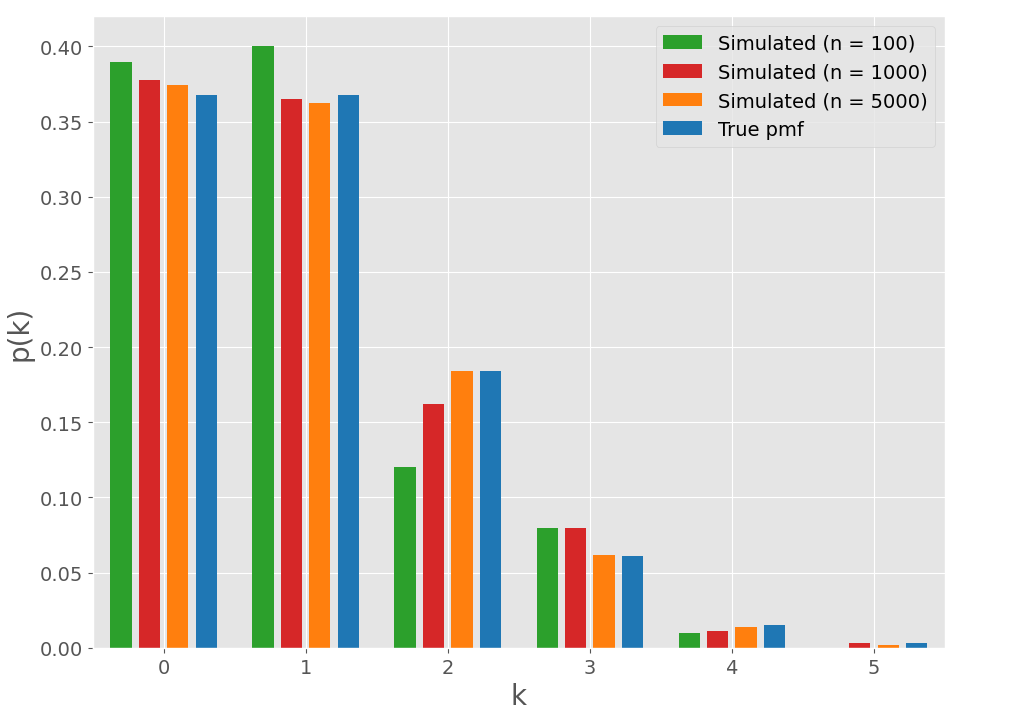
\includegraphics[scale=0.5]{fig/img/poisson.png} 
        \caption{Den simulerede relative frekvens af $k = 0, 1, \ldots, 5$ og den rigtige pmf.}
        \label{fig:simuleringAfPoisson}
    \end{figure}
    Det kan umiddelbart ses at den simulerede relative frekvens af $k$ går imod $p(k)$, når $n$ vokser.
\end{exmp}



% Input-filer bør opdeles således, at hver fil svarer til et kapitel. Makroen
% \include indsætter et sideskift og indholdet fra den givne stil.

% \include{incl/main/example1}
% \include{incl/main/example2}
% ...

% Appendicer indsættes inde i en appendices-blok og bliver nummereret med
% bogstaver i stedet for tal
\begin{appendices}
\chapter{Prædikat}
\begin{defn}
         Hvis en udtalelse indeholder en fri variable, så kaldes det for et prædikat om elementerne i en givet mængde. 
\end{defn}
%http://web.math.ku.dk/noter/filer/dis2013.pdf

\chapter{Kode til simulering af diskrete stokastiske variable} \label{app:kodeTilSimuleringAfDiskreteVariable}
\lstinputlisting[
    firstline=2,
    lastline=63,
    label={code:dsv}
    caption={Kode til at simulere diskrete stokastiske variable og til eksempel \ref{exmp:simuleringAfDiskreteVariable}}
]{code/poisson.py}
\end{appendices}


% Dokumentets 'back matter' er til ekstra ting som f.eks. litteraturlisten.
% Overskrifter bliver ikke nummereret her.
\backmatter

% Automatisk litteraturliste baseret på, hvilke kilder, der er blevet refereret
% til i løbet af rapporten.
\bibliographystyle{apalike}
\bibliography{
  incl/bib/books,
  incl/bib/articles,
  incl/bib/software
}
\end{document}
